\documentclass[a4paper,12pt]{article}


\usepackage{lscape}
\usepackage{pbox}
\usepackage{tabularx}
\usepackage[parfill]{parskip}
\usepackage{graphicx}
\usepackage{booktabs}
\usepackage{listings}
\lstset{
    escapeinside={(*}{*)},
    breaklines =true
}
\usepackage{multirow}

\title{AutoRSpec}
\date{2017-04-25}
\author{Dan Shreeve}

\begin{document}

\pagenumbering{roman}
\addcontentsline{toc}{section}{Title page}
\maketitle

\newpage
\addcontentsline{toc}{section}{Signed declaration}
\section*{Signed declaration}
All sentences or passages quoted in this report from other people's work have been specifically acknowledged by clear cross-referencing to author, work and page(s). Any illustrations which are not the work of the author of this report have been used with the explicit permission of the originator and are specifically acknowledged. I understand that failure to do this amounts to plagiarism and will be considered grounds for failure in this project and the degree examination as a whole.
\par Name: Daniel Demaine Shreeve
\par Signature: .................................
\par Date: 03/05/2017

\newpage
\addcontentsline{toc}{section}{Abstract}
\begin{abstract}
Software Testing benefits the development and maintenance of a system by increasing quality and reliability. Software Testing also contributes around half of the cost of producing a system. Automating part or whole of this process reduces the cost whilst maintaining the benefits. The aim of this project is to produce a system that automatically generates RSpec test cases for model validation in Ruby on Rails. The tests will be generated from a formal database specification that the user has defined using the system. A file can be generated and inserted into the user's application and run as though they had been written by the user. The time taken to insert the necessary information should be less than the time taken to write the tests manually, otherwise the user will not benefit.
\end{abstract}

\newpage
\addcontentsline{toc}{section}{Acknowledgements}
\section*{Acknowledgements}
First and foremost I would like to thank my supervisor \textbf{Dr. Gordon Fraser} for accepting my proposed project and providing impeccable advice and guidance throughout the process.
\par Finally I would like to thank my parents, \textbf{Linda Shreeve} and \textbf{Paul Shreeve}, and my grandparents \textbf{Elsie Marsden} and \textbf{Ray Marsden} for giving me the oppurtunity to go to university and supporting me throughout.

\newpage
\tableofcontents

\newpage	
\pagenumbering{arabic}
\section{Chapter 1: Introduction}

\par How severe can the consequences be from an error in a piece of software? In 1983 a bug in a piece of software almost started World War Three.
\vspace{3mm}
\par During the Cold War, tensions between the US and Soviet Russia were extremely high. A Soviet early warning system had detected the launch of five ballistic missiles from the US. The only reason that Soviet Russia did not retaliate, thereby starting World War Three, was the fact that Lt Col Stanislav Petrov had a "...funny feeling in my gut"\cite{ZDNetDisasters} and concluded that if the US was launching a full scale attack they would launch more than five missiles. The error in the system was discovered to be a bug in part of the software that distinguished false missiles from satellites picking up the reflection of sunlight from the top of clouds.\cite{ZDNetDisasters} If the bug in the code had falslely detected more missiles the world could be a very different place today.
\vspace{3mm}
\par Software testing increases the relability of a system and quality, by detecting errors and bugs which can be fixed, quality can aslo be further improved by tests proving that the system meets its design requirements. However, software testing is very costly, accounting for half the time put into development of a system and half of total expenditure.\cite{myers2011art} By automating part or all of the software testing process, testing costs can be reduced, whilst maintaining the benefits.
\vspace{3mm}
\par The motivation for this project is to bring the benefits of automated testing to Ruby on Rails. Ruby on Rails is a web application framework that allows developers to create fully functioning applications in a short of space of time. The reduction in time spent implementing increases the proportion of time spent testing. Thefore Ruby on Rails would benefit greatly from automated testing. This would further enhance the time saving feature of Ruby on Rails.
\vspace{3mm}
\par This project aims to create a system that Ruby on Rails developers can use to reduce the development time of their projects by automatically generating all or part of the tests they require. The tests generated should not reduce the reliability and quality that manually written tests create.

\par \textbf{Chapter 2: Literature Review and Research} gives detailed background information on software testing and how it can be automated. It then follows how testing can be carried out in Ruby on Rails applications with a couple examples of existing teset automation in Ruby on Rails. Finally the chapter discusses the tools that will be used to construct this project.
\par \textbf{Chapter 3: Requirements and Analysis} discusss how the motivation is refined into a more spefici aim and gives the objectives and requirements that the project should have to achieve this aim.
\par \textbf{Chapter 4: Design} outlines the design of the project. Discussing and demonstrating vaarious aspects such as the database and value generation.
\par \textbf{Chapter 5: Implementation and Testing} shows how the design was implemented in detail broken down into sections on setup, database, value generation, test case templates and the overall test suite layout. It then shows how the project was tested and how the requirements from chapter 3 are met.
\par \textbf{Chapter 6: Results and Discussion} evaluates the project and discusses how effective the final implentation is against its aim.
\par \textbf{Chapter 7: Conclusions} discusses various ways in which the system could be improved and its potentail to be expanded. Then is wrapped up with a conclusion on the project as a whole.





\newpage
\section{Chapter 2: Literature Review and Research}




\subsection{Testing and Automation}
\par The European Space Agency spent ten years and \$7 billion designing and constructing the Ariane 5, a rocket that can launch multiple satellites into orbit from a single launch. Thirty nine seconds into its maiden voyage it exploded, destroying the Ariane 5 and its cargo of four uninsured, extremeley expensive scientific satellites. The explosion was caused by its own self-destruct sequence which was triggered automatically as the boosters were being torn away by aerodynamic forces. These extreme forces were caused by the rocket trying to recorrect its course in response to flight data provided by the guidance system. The guidance system, along with its backup, had crashed and shutdown. The flight data provided, that caused the rocket to readjust its course, was actually a diagnostic error message. 
\vspace{5mm}
\par The cause of the shutdown was the guidance system trying to convert the sideways velocity of the rocket from 64-bit to 16-bit. To make matters worse, the programmers were aware that it could overflow but assumed that the particular causal variable would never be large enough, as it was used to prepare for launch and not in flight. However it was decided the system should run into the first forty seconds of flight, in case of a brief hold in the launch countdown, to make restarting the system easier. A known flaw in a system, that could have been handled, resulted in a chain of events that led to the catastrophic explosion of Ariane 5.\cite{Ariane5}.
\vspace{5mm}
\par Software disasters can be caused by poor testing practices\cite{mcquaid2012software}, if the correct testing procedures and practices had been in place for both Ariane 5 and the Soviet Guidance System example from the Introduction these situations could have been avoided. Software testing is therefore extremely important and should be included in the development of all software applications. What is software testing and how does it help avoid these situations ?
\vspace{5mm}
\par Software testing is an investigation into a piece of software that provides information during development and maintenance. A process or series of processes are carried out that are designed to make sure computer code does what it designed to do and is absent of unintended behaviour\cite{myers2011art}. The information retrieved from the proccesses can be used to track the progress during development against acceptance criteria and detect and locate errors and bugs. Errors and bugs detected within the code of the are immediatley known and can be handled, providing a smoother and more consistent development and maintenance flow. Software testing provides a more reliable and higher quality product when used as part of the development process due to these benefits.
\vspace{5mm}
\par Testing however can not guarantee that a program or peice of code is without errors, therefor completing testing is impossible. This is why the design of tests is vital to the integrity of the testing, making the tests as complete as possible. Given the constraints on time and cost, effective testing is simply "What subset of all possible test cases has the highest probability of detecting the most errors?"\cite{myers2011art}. Tests are designed using information about the program along with its intended behaviour. In a given environment, with proper determined input, there is an expected behaviour/output. If the code under test does not display the desired outcome it is said to have failed the test. 
\vspace{5mm}
\par A 'test case' will test a very specific behaviour of a program. A collection of test cases is a 'test suite', representing that a certain section of the system has a specificied set of behavoiurs. A relevant example would be for a table in a database. The test suite would represent if the table has the desired validations in place and would consist of test cases that tested each specific behaviour in isolation. The tests would be run as a set to confirm the table has the desired behaviour. When undesired behaviour is detected the test result will highlight the exact error in the code. The design of these test cases is crucial. To design these cases information is required, this information is sourced in two main ways Functional and Structural.
\vspace{5mm}
\par  Functional Testing also known Black-box testing, is the technique of creating test cases with information from a formal or informal functional specification. A functional specification is the description of intended program behaviour distinct from the program itself. The software requirements and or its design specification are most commonly used to derive the functional specification. The software entity under test is treated as a black box, the actual code implementation is not known, where proper inputs are fed in and the output is observed. If the output or behaviour is that specified in the specification the test has been passed, otherwise it has been failed. Example: When a user clicks the Home tab in the nav bar they are directed to the Home page, in this case the input is the user clicking the home tab and the desired behaviour is being directed to the home page. Black box testing can detect some faults that white box cannot, such as absent behaviours that are in the functional specification of requirements but not coded into the software application in error. The systematic nature of Black-box testing can help avoid missed test cases and provide more consistent coverage.\cite{nidhra2012blackbox}\cite{young2008software}
\vspace{5mm}
\par One approach to functional testing is a systematic approach. A systematic approach has four steps :\cite{young2008software}
\vspace{5mm}
\begin{enumerate}
\item Partition the functional specification into independently testable features using a divide and conquer approach. For example, for a database table, dividing a table in a databse into its fields, then dividing again into the properties of each field. 
\item For each independently testable feature find a representative class of values or derive a model to test it. For a string field with property of length greater than five. We may derive a specail case of blank string, a string of length less than five and string with length greater than five.
\item Generate test case specifications. Finding concrete values for the reprensentive class of values or model above. Building on the previous example we may have \{ "", "less" ,"longer"\}
\item Generate test cases and institute tests, turning specifications into tests and instituting them.
\end{enumerate}
\vspace{5mm}
\par Structural testing, also known as White box testing. uses the physical implementation of the software itself such as source code as information to produce test cases. A common approach to white box testing is 'Control Flow' testing. Due to the nature of code varying greatly between projects and the complexity and detail that can be involved the following steps have been simplified whilst maintaining the core principle.
\vspace{5mm}
\begin{enumerate}
\item Identify a feature to be tested. This could be on a small or large scale, for our examples we will choose creating an entry on a database.
\item Create a flow graph plotting all steps and paths the feature can execute, this would include steps such as verification.
\item Identify paths through the flow graph, entry is created successfully and displayed or unsuccessfuly and prompted with an error message.
\item For each path write a test case that is expected to execute this path, with valid variables an entry should be created and it should be displayed.
\end{enumerate}
\vspace{5mm}
\par Software testing is necessary and very costly. "In a typical programming project approximately 50 percent of the elapsed time and more than 50 percent of the total cost were expended in testing the program or system being developed"\cite{myers2011art}. Reducing the costs, both time and monetary, is the main motivation for Automated Testing. Another overlooked and unappreciated benefit of automating testing is that test case generation is one of the most intellectully demanding and critical challenges in software testing.\cite{anand2013orchestrated} By automating this process it not only reduces costs but also allows developers to dedicate more time and effort to other areas, also in some cases it is harder to create a test case but easy to verify a generated test case is correct. A whole systems tests do not have to be automatically generated to reduce costs and benefit.
\vspace{5mm}
\par An Automated functional testing approach follows the same methodology as manual systematic generation of test cases. Each step is automated and follows the same principles. The information as before used to derive test cases is the functional specification. The functional specification is however only formal  and has specified syntax so that it can be interpreted by the system that will generate the test cases. There is more creativitivy and design put into the functional specification as the test designer is usually limited to a choice of test selection criteria. For step 3 the system must also include value generation that can meet the representative class of values outlined in step 2.\cite{young2008software}
\vspace{5mm}
\par Automated functional testing tends to be more complex, as it has to understand and interpret human written code. One method that has recieved alot of attention from researchers and is Symbolic Execution. This approach is similar to that of Control Flow, where symbolic values, instead of concrete values, are used instead for program inputs. Programs variables are described by the symbolic expressions of those inputs. The state of the program includes the symbolic values of program variables, a program counter and the path contraint on symbolic values: a boolean formula over the symbolic values input. Using this method it can explore all possible path divergences through a system and identify stop points, where the path ends. The major problem with automated White-Box testing is identifying if a behaviour, stop point or a specific divergence in Symbolic execution, is desired or not. This problem is known as the Oracle problem, as desired behavoiur of code is contained within its specfication and design, not its implementation. Therefore some level of user input is required.\cite{anand2013orchestrated}
\vspace{5mm}
\par Another relevant challenge for Symbolic Execution is developing a system that can cover multiple languages at once. This is very complex and producing a system can produce feasible output can be impossible due to the path divergence problem, where, either a user has to specify so many models automation is not feasible, or it doesnt find a signifcant amount of feasible program paths. As Ruby on Rails design environment can vary drastically between projects due to the flexibility of its framwork and use of Gems I will only consider and that some level of User input is required I will only consider Black Box testing techniques when I come to designing the project. This will deliver a product that will be usable to a wider audience as it is dependent upon on specification for which I can define. Interpreting multiple languages and being flexible enough to be useful is out of the scope of this project.
\vspace{5mm}
\par PARAGRAPH SAYING BB CHOSEN SO VALUE GENERATION NEEDS TO BE CONSIDERED WHEN CHOOSING TOOLS

\subsection{Testing in Rails}

\par Ruby on Rails applications are primarily developed using the generation of skeletons with variables set by the developer. The skeletons save a vast amount of time by generating a default environment which can then be built upon according to the section under development. By default one of the files created is a test file and it uses the Ruby on Rails MiniTest class.\cite{railsTest}

\par TEST UNIT

\par RSPEC

\par CONCLUDE RSPEC

\par RSPEC IN GREATER DETAIL (may be few par)

\par TEMPLATES FOR RSPEC - NEED STRING MANIPULATION ETC

\par FACTORY GIRL



\subsection{Tools to use}
\par TOOL REQUIREMENTS FROM PREVISOUS SECTIONS
\vspace{5mm}
\par An MVC web application fits all these criteria. MVC, Model-View-Controller is an architectural pattern that seperates an application into three interconnected parts. This separation (of the three components) allows for responsibilities to be allocated independently to each component, seperating the logic from the user. The model is responsible for the data of the application and the rules and logic used to create and update the information. The view is responsible for displaying the data and possible interactions with the system to the user. The controller is responsible for controlling the flow of the system,  accepting user input and converting it into commands for the model and view.
\vspace{5mm}
\par An example of the components interacting would be creating an entry to a database. The "view" would be responsible for displaying the form in which to fill in. On submission the "controller" will process the information, ensure only persmissable information is submitted and enter additional information, then send it to the "model". The model will verify the structure of the information, ensure the correct fields are present and accord with its rules. The model will then notify the controller if the submission was successful or not and the controller will update the view to reflect the status.
\vspace{5mm}
\par This seperation of components means that all user interaction with the database has to go through the controller and is therefore limited to what the developers want users to be able to do. This provides a high level of security as each action is controlled and the internal structure and representation of the information within the database is hidden. Simultaneous development is also possible due to the seperation of the components, work on the front and back end concurrently. Although I will not be able to get the full benefit of this aspect (as I am developing the project solo), it will allow me to shift focus as components do not need to be finished when switching from one to another, giving greater flexibility in development. 
\vspace{5mm}
\par High levels of cohesion are inherited automatically from the architecture with the grouping of logically similar elements, this makes the code easier to read and creates a more natural flow within the source code. There are however some drawbacks to MVC architecture, they are inherently more complex due to the seperation and the framework must be learned. Also there may be multiple programming languages involved. This steep learning curve could mean a large initial investment (time/cost) into a development team to learn a new framework and new languages.
\vspace{5mm}
\par MVC web application frameworks have become extremely popular and are behind some of the most used and powerful websites. Django an MTV, follows MVC architecture but its creators decided to rename the components \cite{Django} to better suit them, is behind the two most visted websites in the world Google and YouTube\cite{SHUUP}\cite{Alexa}. Ruby on Rails another MVC is behind Twitter, Airbnb and Soundcloud.\cite{Coderfactory} MVC frameworks are known for their scalablity, being suitable for the smallest to the largest projects. However FaceBook decided that its scalablity had reached its limit, that adding new features made the code exponentailly more complex.\cite{Infoq} My project will be no where near the scale of facebooks sourcecode so I do not need to worry about reaching the end of its scalibilty.
\vspace{5mm}
\par The chosen MVC to construct the project in is Ruby on Rails. I have done previous projects in both Ruby and the Rails framework, the rest of this section will show that Ruby on Rails is an adequate choice.
\vspace{5mm}
\par Ruby was selected as the primary programming language by default as it is the language that runs Ruby On Rails. Ruby is a dynamic, multi-paradigm programming language. The paradigms consist of Object-oriented, Imperative, Functional and Reflective making it a very powerful and versatile language. This combination is from its founder ‘Yukihiro Matsumoto’ who was influenced by Perl, Smalltalk, Eiffel, Ada, and Lisp.
\vspace{5mm}
\par Ruby’s primary design goal was to “make a language that he himself enjoyed using, by minimizing programmer work and the potential for confusion”(Ruby Wiki). Achieved with a focus on human interaction, how programmers code and design applications as opposed to focusing on how the code will run on machines. And also following the principle of least astonishment, where the behaviour of the language minimizes confusion for experienced users.
\vspace{5mm}
\begin{figure}
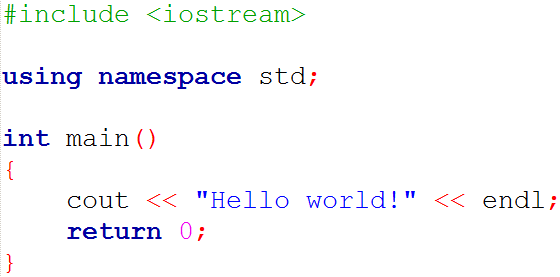
\includegraphics[width=\linewidth]{screenshots/c++_hello_world}
\caption{C++ print Hello world to console}
\label{fig:c++print}
\end{figure}
\begin{figure}
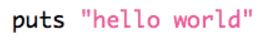
\includegraphics[width=\linewidth]{screenshots/ruby_hello_world}
\caption{Ruby print Hello world to console}
\label{fig:rubyprint}
\end{figure}
\par The above two images show C++ \ref{fig:c++print} and Ruby \ref{fig:rubyprint} printing ‘Hello world’ to the console. The comparison between the two languages highlights the efficiency and simplicity of the Ruby language.Ruby on Rails projects are commonly worked on by a group of people and in multiple languages, therefore the simplistic syntax gives greater clarity and understandability to programmers who are lesser experienced in Ruby.\cite{AboutRuby}
\par Ruby is open source, free and redistributable with a vast range of existing code from both Ruby and its large community. Primarily consisting of Gems, code packages that can be installed and supported into a project easily and with minimal effort via RubyGems, and frameworks, such as Ruby on Rails. Making it very popular for education and business. Following the DRY ‘Don't Repeat Yourself’ principle in a very effective and efficient manner.\cite{AboutRuby}
\par Ruby was ranked ninth on TIOBE index\cite{TOBIE} and has become a very popular and respected language relative to its age among the other languages on the index. No alternatives could be considered due to the dependency of Ruby on Rails on Ruby, however Ruby is a very strong and durable language so it does not detract from the overall project.
\vspace{5mm}
\par FORMS AND DATABASE SUPPORT FOR INPUTTING INFORMATION THAT CAN BE PROCESSED
\vspace{5mm}
\par STRING MANIPULATION FOR TEMPLATES
\vspace{5mm}
\par NUMBER GENERATION
\vspace{5mm}
\par STRING GENERATION FROM REGEXP USING GEM REGEXP.RANDOM
\vspace{5mm}
\par RUBY HAS NECESSARY LOGIC TO CONTROL FLOW ETC


\subsection{Evaluation}
\par HOW TESTS ARE EVALUATED
\par HOW OTHER PEOPLE EVALUATED PROJECTS
\par INJECTION
\par DOG FEED
\par COMPARE OUTPUT WITH WHAT EXISTING HAD
\par COMPARE CODE COVERAGE
\par TIME SAVED


\newpage
\section{Chapter 3: Requirements and Analysis}

\par This project started with the motivation of bringing automated testing to Ruby on Rails. From research carried out and disscussed in Chapter 2 and considering the scale of the project the way to achieve this was to focus on validation in the model component and produce RSpec test cases. A more precise description of the project is therefore \textbf{To create a system that automatically generates RSpec test cases for model validation in Ruby on Rails Applications}. To accomplish this aim there are three main aspects to the system, as follows:

\begin{enumerate}
\item Allow a user to create and maintain a formal specifcation
\par A user should be able to describe all tables, fields and corresponding validation properties using the system. The user should also be able to edit and update the formal specification due to their changing demands.
\item Generate a valid RSpec test case
\par The RSpec test case should be generated with information entered from defined formal specification. To be valid the RSpec test case must meet certain critera. The test case must run the same as a manually produced user test case. It must only test the specified behaviour, e.g Employee table, Age field, must be greater than 18, and nothing else. It must produce a human readable test case with a human readable  behaviour descriptor that makes the user aware of exactly what behaviour has failed. It must produce a generated value that isolates the behaviour under test, it generates a value that fails the validation under test while passing the other validations for the field.
\item Consolidate all RSpec test cases for to make a valid test suite for a table
\par All test cases for a table, for all its fields and assigned validations, must be consolidated into a test suite that runs as a manual written test suite.
\end{enumerate}

\par To make the system viable and useful to developers there are some additional considerations
\begin{enumerate}
\item Ease of use
\par The system built should be easy and intuitive to use. 
\item Time saving
\item Creating the formal specification must take less time than it takes to write the tests manually
\end{enumerate}

\par Ruby on Rails has fourteen data types supported natively be ActiveRecord\cite{railsTableType}. Ruby on Rails also has many active record validations supported natively. To fit the scope of the project not all data types and validations will be supported. The selection of data types and validations supported are as follows.

\par Data Types Supported
\begin{enumerate}
\item Integer
\item Float
\item String
\end{enumerate}

\par Integer and Float Validations
\begin{enumerate}
\item Greater than
\item Greater than or Equal to
\item Equal to
\item Less than or Equal to
\item Less than
\item Other than
\item Divisible by
\item Blank
\item Inclusion
\item Exclusion
\end{enumerate}

\par String Validations
\begin{enumerate}
\item Maximum Length
\item Minimum Length
\item Exact Length
\item Format
\item Blank
\item Inclusion
\item Exclusion
\end{enumerate}


\begin{table}
\centering
\caption{Formal Specification Requirements}
\label{req:1}
\begin{tabularx}{\textwidth}{|l|X|l|}
\hline
\textbf{ID} & \textbf{Requirement}                                                   & \textbf{Priority} \\ \hline
\textbf{1}  & A user can create a Project                                            & \textbf{M}        \\ \hline
\textbf{2}  & A user can edit a Project                                              & \textbf{M}        \\ \hline
\textbf{3}  & A user can delete a Project, associated Tables are also deleted        & \textbf{M}        \\ \hline
\textbf{4}  & A user can create a Table, only for a given  Project                   & \textbf{M}        \\ \hline
\textbf{5}  & A user can edit a Table                                                & \textbf{M}        \\ \hline
\textbf{6}  & A user can delete a Table, associated Fields are also deleted          & \textbf{M}        \\ \hline
\textbf{7}  & A user can create a Field, only for a given Table                      & \textbf{M}        \\ \hline
\textbf{8}  & A user can edit a Field                                                & \textbf{M}        \\ \hline
\textbf{9}  & A user can delete a Field, associated validations are also deleted     & \textbf{M}        \\ \hline
\textbf{10} & A user can assign a validation, only for a given Field       & \textbf{M}        \\ \hline
\textbf{11} & A user can only create a value for a assigned validation                  & \textbf{M}        \\ \hline
\textbf{12} & A user can edit a  value                      & \textbf{M}        \\ \hline
\textbf{13} & A user can view all Projects                 & \textbf{M}        \\ \hline
\textbf{14} & A user can view all Tables associated to a given Project               & \textbf{D}        \\ \hline
\textbf{15} & A user can view all Fields associated to a given Table                 & \textbf{D}        \\ \hline
\textbf{16} & A user can view all validations and values associated to a given field & \textbf{D}        \\ \hline
\end{tabularx}
\end{table}

\begin{table}
\centering
\caption{RSpec Test Case Requirements}
\label{req:2}
\begin{tabularx}{\textwidth}{|l|X|l|}
\hline
\textbf{ID} & \textbf{Requirement}                                                                                                                       & \textbf{Priority} \\ \hline
\textbf{1}  & RSpec test case should be runnable                                                                                                         & \textbf{M}        \\ \hline
\textbf{2}  & RSpec test case should only test one behaviour                                                                                             & \textbf{M}        \\ \hline
\textbf{3}  & RSpec test case must should test behaviour intended                                                                                        & \textbf{M}        \\ \hline
\textbf{4}  & RSpec descriptor must be human readable                                                                                                    & \textbf{D}        \\ \hline
\textbf{5}  & When test case fails, its output must specify exact behaviour at fault                                                                     & \textbf{D}        \\ \hline
\textbf{6}  & RSpec test case should have human readable syntax                                                                                          & \textbf{D}        \\ \hline
\textbf{7}  & Be able to generate an Integer that satisfies all validations and their values assigned to a field                                         & \textbf{M}        \\ \hline
\textbf{8}  & Be able to generate an Integer that does not satisfy a validation but satisfies all other validations and their values assigned to a field & \textbf{M}        \\ \hline
\textbf{9}  & Be able to generate a Float that satisfies all validations and their values assigned to a field                                            & \textbf{M}        \\ \hline
\textbf{10} & Be able to generate a Float that does not satisfy a validation but satisfies all other validations and their values assigned to a field    & \textbf{M}        \\ \hline
\textbf{11} & Be able to generate a String that satisfies all validations and their values assigned to a field                                           & \textbf{M}        \\ \hline
\textbf{12} & Be able to generate a String that does not satisfy a validation but satisfies all other validations and their values assigned to a field   & \textbf{M}        \\ \hline
\end{tabularx}
\end{table}

\begin{table}
\centering
\caption{RSpec Test Suite Requirements}
\label{req:3}
\begin{tabularx}{\textwidth}{|l|X|l|}
\hline
\textbf{ID} & \textbf{Requirement}                                          & \textbf{Priority} \\ \hline
\textbf{1}  & RSpec test suite should be runnable                           & \textbf{M}        \\ \hline
\textbf{2}  & RSpec test suite should be contain all test cases for a table & \textbf{M}        \\ \hline
\textbf{3}  & RSpec test cases should be grouped via field                  & \textbf{D}        \\ \hline
\textbf{4}  & RSpec test cases should be in a logical order                 & \textbf{D}        \\ \hline
\textbf{5}  & RSpec test suite must be available for download               & \textbf{M}        \\ \hline
\end{tabularx}
\end{table}

\newpage
\section{Chapter 4: Design}

\subsection{Database}
\par The database was designed to accomodate the formal specification and extra information needed for RSpec test cases. Ruby on Rails has native support for relations via ActiveRecord, this provided flexibility in being able to have many relations. The design paradigm of sole responsiblity was carried forward and each table has one purpose.

\begin{figure}
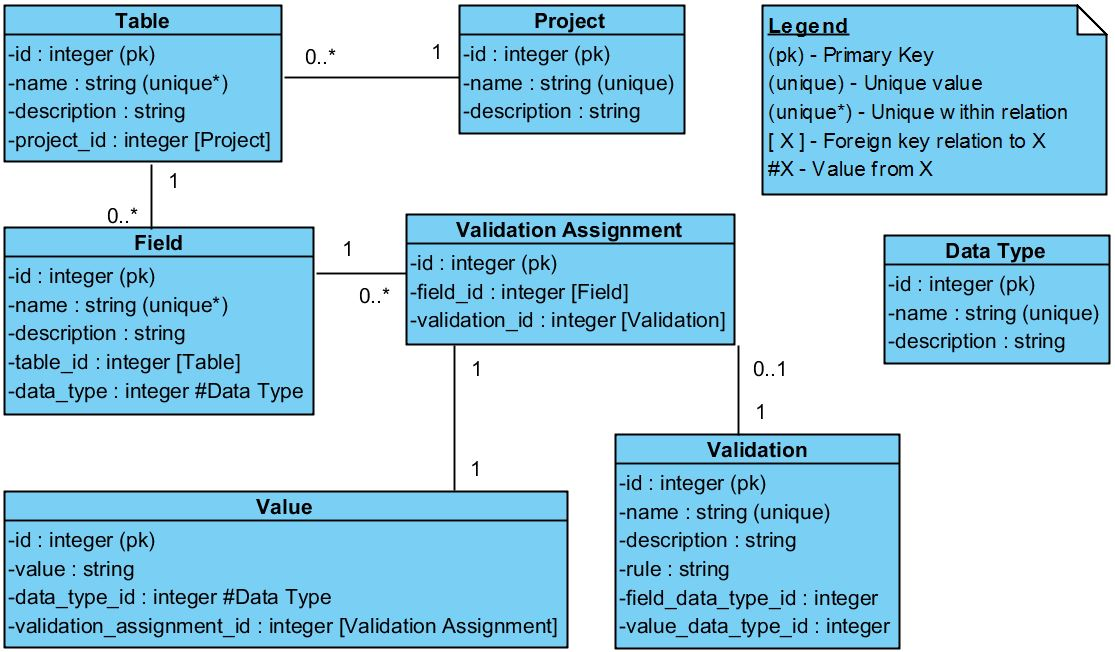
\includegraphics[width=\linewidth]{screenshots/databaseUML}
\caption{UML Database diagram}
\label{fig:UML1}
\end{figure}

\par \textbf{Project}
\par Project allows for a user to use the system for multiple projects, that is to organise groups of tables that are disconnected. The name field is unique to avoid confusion amongst projects. The description field is only for the user to add extra information if they desire and serves no functional purpose in the system. A project can have zero to many tables. When a project  is deleted its associated tables should also be deleted.

\par \textbf{Table}
\par Table is the table in a user's database for which they are constructing a functional specification. A table can only be created with a valid project\_id foreign key. The name is unique within the scope of the project, multiple tables can exist with the same name within the database but they must belong to seperate projects. The description field is only for the user to add extra information if they desire and serves no functional purpose in the system. A table belongs to a project and has zero to many fields. When a table is deleted its associated fields should also be deleted.

\par \textbf{Field}
\par Field is the field in a user's database for which they are constructing a functional specification. A field can only be created with a valid table\_id foreign key. The name is unique within the scope of the table, multiple fields can exist with the same name within the database but they must belong to seperate tables. The description field is only for the user to add extra information if they desire and serves no functional purpose in the system. Data\_type\_id is the fields data\_type and is limited to values in the Data Type table, however no relation is forced. A field belongs to a table and has zero to many Validations through Validation Assignments. When a table is deleted its associated validation assignments should also be deleted.

\par \textbf{Validation}
\par Validation is a validation the user can associate to a field. The user can not create, edit or destroy these and they are seeded in the database. The name is unique within the scope of its field\_data\_type. The description field is to aid the user in understanding what the validation is. The rule field is used within the system to generate values. Field\_data\_type\_id and value\_data\_type\_id limited to values in the Data Type table, however no relation is forced, and are used so only appropriate validations can be assigned to fields. A validation has zero to many fields through validation assignments.

\par \textbf{Value}
\par Value is the value of a validation that a user associates with a field, E.g false for blank or ten for minimum length. A value can only be created with a valid validation\_assignment\_id foreign key. The value is stored as a string and the data type of which the system should treat the value as is stored in data\_type\_id, which refers to the data type table, but no relation is enforced. A value belongs to a validation assignment.

\par \textbf{Validation Assignment}
\par Validation assignment associates a field with a validation and also the value for that validation. The assignment is created then a value is created belonging to the assignment. A validation assignment can only be created with both valid field\_id and validation\_id foreign keys. A validation assignment has one field, one validaiton and owns a value.

\par \textbf{Data Type}
\par Data type is used to provide consistency throughout the system by checking data types are equal between entities, checking values of are the correct type and also used in forms to reduce options available to the user. The user can not create, edit or destroy these and they are seeded in the database. The name field is unique to avoid confusion amongst data types and avoid possible duplication. The description field is to inform the user on the data type. Data  type has no relations, but is used throughout the system in reference.


\subsection{View and Flow}
\par The main consideratons when designing the look and how the user navigates and uses the system were human-centered design principles with the goal of increasing effectiveness, efficency and satisfaction\cite{maguire2001methods} .The principles taken into consideration and how they were applied are\cite{abras2004user}:

\begin{enumerate}
\item \textbf{Simplifying the structure of tasks}
\par An average user is able to remember five things at a time. Providing consistency within similar methods such as creation of entitys and also clearly displaying where in the system the user is reduces the strain on both long and short term memory. The creation, deletion and editing of entitys follows the familiar and consistent method of filling in a form and submitting it. At the top of each page it clearly displays how deep in the system and also the names of each level. This means the user will have to remember less when using the system.
\item \textbf{Exploiting the power of constraints}
\par Reducing and not exposing a user to redundant or irrelevant information allows a user to use a system more efficently and with less effort, by not having to process such information. This is used by displaying only the related entities when viewing an entity, only the fields for a table are shown when viewing that table. When a user is creating an entity with a form options are reduced to those that are valid, only choose from Integer validations for a Integer field. Entitys that are dependent on a another, field is dependent on table, are only available to create when viewing the dependent upon entity.
\item \textbf{Make things visible}
\par Bridging the gulf of execution, buttons and links do what a user expects them to do.  This principle followed by using standard naming conventions on standard objects such as buttons and links that a user is familiar with.
\end{enumerate}

\begin{figure}
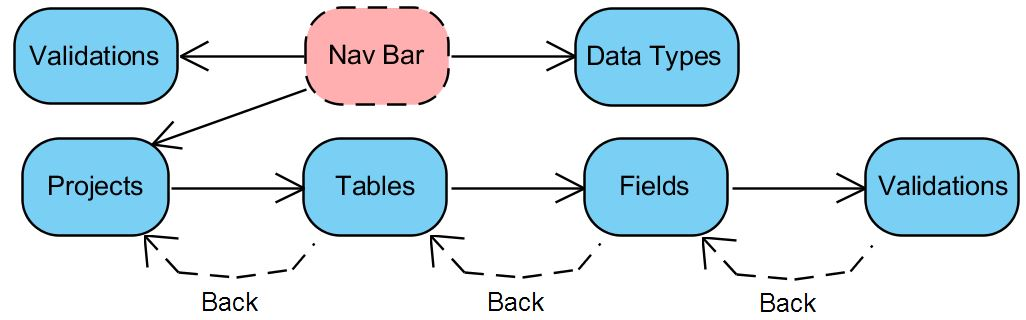
\includegraphics[width=\linewidth]{screenshots/pageflow}
\caption{The navigational flow of the system}
\label{fig:nflow}
\end{figure}


\begin{figure}
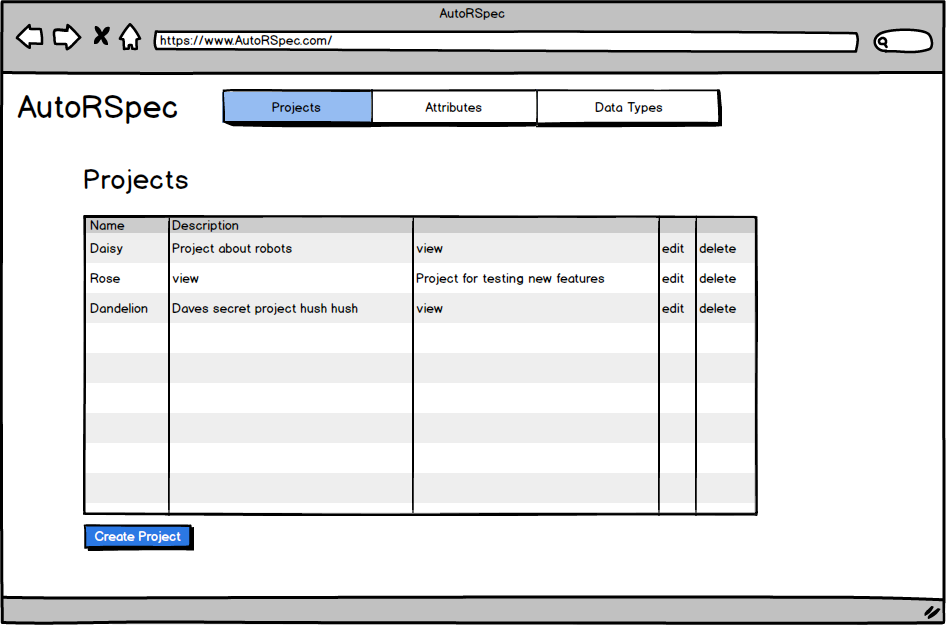
\includegraphics[width=\linewidth]{screenshots/muhome}
\caption{Mock up of projects page for the system, also home page. }
\label{fig:mu1}
\end{figure}

\begin{figure}
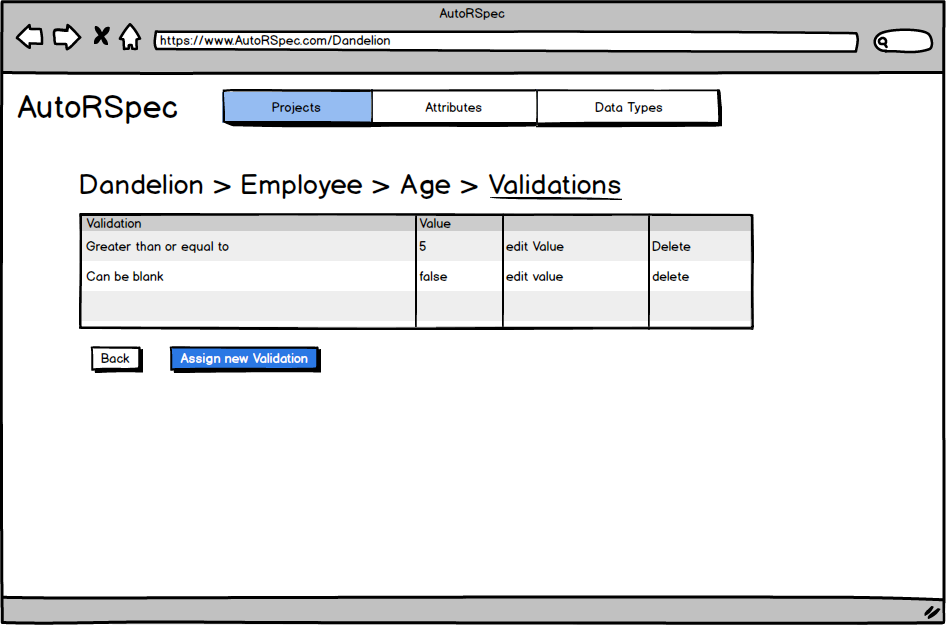
\includegraphics[width=\linewidth]{screenshots/mutable}
\caption{Mock up for a table in the system displaying its fields}
\label{fig:mu2}
\end{figure}

\begin{figure}
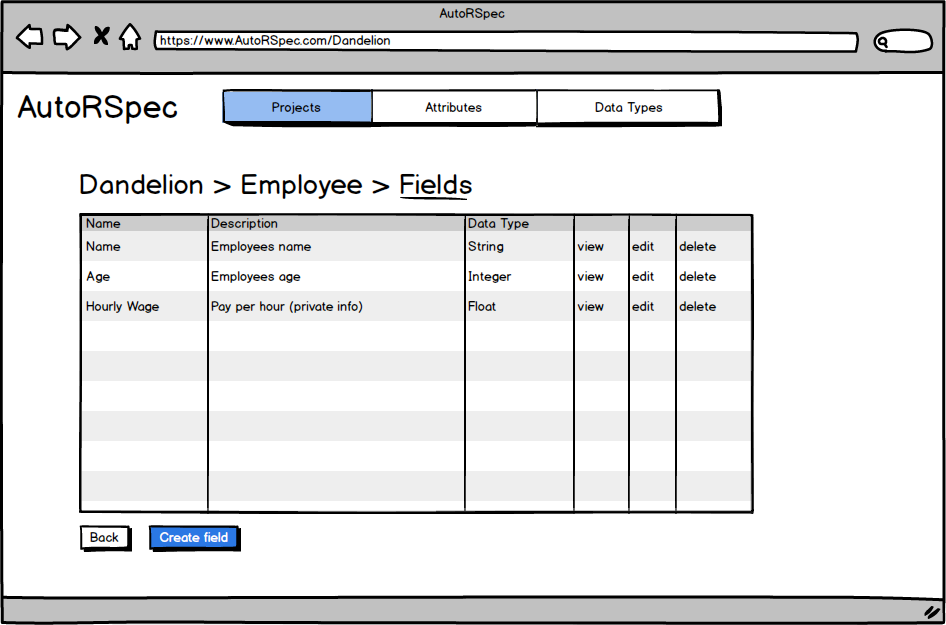
\includegraphics[width=\linewidth]{screenshots/mutablefields}
\caption{Mock up for a field in the system displaying its validation}
\label{fig:mu3}
\end{figure}

\begin{figure}
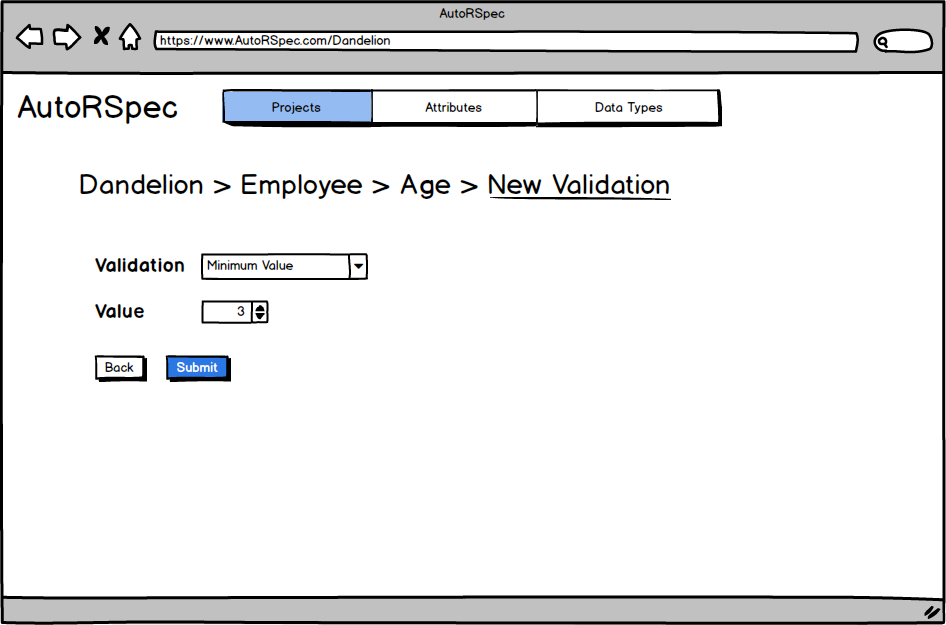
\includegraphics[width=\linewidth]{screenshots/muform}
\caption{Mock up for a form in the system}
\label{fig:mu4}
\end{figure}

\par \textbf{General}
\par Consistency was at the the forefront of the visual and flow design. Each page that has a dependent entity can only be created via a button on the page of that entity\ref{fig:mu2}. When viewing an entity it will display all and only its dependent entities in a table.\ref{fig:mu2} The dependent entites can be viewed, edited and deleted from this table via links in the row of that entity on the table\ref{fig:mu3}. Each page that is dependent upon on entity can access the dependent enity via the back button\ref{fig:mu3}, also applies naviagtionally to forms\ref{fig:mu4}. The header at the top of each page displays the depth the user is at by underlying the current level while also indicating the levels with the name of the entity at that level\ref{fig:mu3}.

\par \textbf{Nav bar}
\par The nav bar is not a page but the navigational bar displayed at the top of each page\ref{fig:mu1}. It links to the projects page, validations page and the data types page via the appropiatley name button.

\par FUNCTIONALITY OF PAGES ???


\subsection{Test Case Generation}
\subsubsection{Value Generation}
\begin{lstlisting}[frame=single,numbers=left,caption= {Pseudo code for value generation} label={psuedo:value}]
generate_value( (*\textbf{isolatedValidation}*), (*\textbf{validations}*))
 for (*\textbf{iterationCount}*) in (*\textbf{1}*) to (*\textbf{X}*)
  (*\textbf{randomValues}*) = generate_random_values (*\textbf{Y}*)
  if (*\textbf{isolatedValidation} not \textbf{nil}*)
   (*\textbf{randomValues}*) = fail_validation((*\textbf{isolatedValidation}*), (*\textbf{randomValues}*))
   if (*\textbf{randomValues}*) is empty
    next
  for (*\textbf{validation}*) in (*\textbf{validations}*)
   randomValues = pass_validation((*\textbf{validation}*), (*\textbf{randomValues}*))
   if (*\textbf{randomValues}*) is (*\textbf{empty}*)
    (*\textbf{next}*)
  if (*\textbf{randomValues}*) is (*\textbf{empty}*)
   (*\textbf{ next}*)
  else
   (*\textbf{return}*) random value from (*\textbf{randomValues}*)
 return (*\textbf{ERROR NO VALUE GENERATED}*)
\end{lstlisting}

\par The psuedo code in Listing 1 shows then general approach to generating a value for a test case. To increase the efficency and speed of potentailly returning a valid value by generating \textbf{X} values at a time for a potentail of \textbf{Y} times. Generating \textbf{X}*\textbf{Y} values initailly will take a greater deal of time and may be overkill. The correct balance will need to be found in implementation of the initail amount of values for each iteration and how many iterations to carry out.
\par The function will take two parameters, a validation to fail and a list of validations to pass. The validation to fail can be nil, in which case it will produce a value that passes all validations in validations parameter. The validations parameter can also be an empty list in which case it will return a value that fails the isolated validation. In the case of nil validation and and empty list of validations or no value can be generated it will return an error.
\par The flow of the function is to generate a random amount of values, then remove those values that pass the isolated validation, afterwards it will remove those that fail each validation in validations. After each time this array of random values is manipulated it will check if its empty, if so it will skip to the next iteration, this improves speed and efficency by eliminating unnesscary operations. When all validations have been processed it will return a random value from random values. The general flow and principles is the same for each data type that values will be generated.


\subsubsection{RSpec Test Case}
\begin{lstlisting}[frame=single,numbers=left,caption= {Pseudo code for value generation} label={psuedo:case}]
it "is (invalid with a value that is not (*\textbf{VALIDATION}*) (*\textbf{VALVALUE}*)" do
  (*\textbf{TABLENAME}*) = build(:(*\textbf{TABLENAME}*), (*\textbf{FIELDNAME}*): (*\textbf{GENVALUE}*)
  if (*\textbf{TABLENAME}*).respond_to?(:valid?)
   expect((*\textbf{TABLENAME}*).not_to be_valid, lambda (*\textbf{TABLENAME}*).errors.full_messages.join("\\n")
 end
end
\end{lstlisting}

\par \textbf{VALIDATION} is the validation that is being tested on the field, and is described as its polar opposite
\par \textbf{VALVALUE} is the value of the validation that is being tested on the field.
\par \textbf{TABLENAME} is the name of the table the field belongs to
\par \textbf{FIELDNAME} is the name of the field under test
\par \textbf{GENVALUE} is the value that will test the validation
\par The RSpec test case template that will be populated with information from the functional specification and value generated. An example of a employees age field with validation of greater than value eight with a generated value of thirteen.

\begin{lstlisting}[frame=single,numbers=left,caption= {Pseudo code for value generation output} label={psuedo:caseex}]
it "is invalid with a value that is not greater than 8" do
  employee = build(:employee, age: (*\textbf{13}*))
  if employee.respond_to?(:valid?)
   expect(employee.to_not be_valid, lambda employee.errors.full_messages.join("\\n")
 end
end
\end{lstlisting}

\subsubsection{RSpec Test Suite}

\par The test suite is responsible for the overall document structure that the user downloads. It will provide the preamble, then iterate through each field and finally end the document. It will provide all necessary logic to navigate test cases correctly and add the correct syntaxical links to the file. 

\begin{lstlisting}[frame=single,numbers=left,caption= {Pseudo code for value generation} label={psuedo:suite}]
require "spec_helper"

desrcibe "(*\textbf{TABLENAMECAP}*)" do
 it "has a valid factory" do
  expect(build(:(*\textbf{TABLENAME}*))).to be_valid
 end
 #for each field belonging to table |(*\textbf{f}*)|
  describe "(*\textbf{f.NAME}*) has property" do
  # genval = generate_value((*\textbf{nil}*), (*\textbf{f.validations}*))
  # add to file test_case_pass_all((*\textbf{f}*),(*\textbf{genval}*))
  #for each validation belonging to (*\textbf{f}*) |(*\textbf{v}*)|
   # genval = generate_value((*\textbf{v}*), (*\textbf{rest of validations}*))
   # add to file test_case((*\textbf{v}*),(*\textbf{f}*),(*\textbf{genval}*))
  #end
  end
 #end
end
\end{lstlisting}
\par EXAMPLE ??
\par To make the pseudo code more clear lines starting with \# are not printed to the document but code that is ran. TABLENAMECAP is the table name capitalised. Lines 1-4 are the preamble and set up the RSpec document and write a test to check the tables factory is valid. Then for each field it will add the correct syntax to the file for that field and follow it by adding a test case to the file that passes all validations. For each validation that field has been assigned it will iterate through isloting each field and adding the relevant test case to the file. Test suite is the top level function therefor before it calls to generate a test case, lines 8,11, it will call the function to generate a valid value for that test case, lines 7, 10. Test suite will finally end the document with the appropiate "end"  syntax that it opened in the preamble.

\section{Chapter 5: Implemention and Testing}


\subsection{Setup}
\par Ruby version 2.1.7 and rails 4.2.5.2 were used to construct this project.
\par Github\cite{github} was used throughout the project to provide version control and to prevent any catastrophes. The airbnb ruby style convention was used to provide clean looking and consistent code\cite{Airbnb}. Rails new was used to instatiate the system. Then the generate scaffolfd command was used to construct the base for each table in the database schema outlined in chapter 4.1 \ref{fig:scaffold}. This sets up the default mvc components for each, the exact files created can be seen in Figure \ref{fig:scaffold}. 
\par Regular expressions are used frequently through the implementation process, to quickly check a regular expression was serving the function expected the Rubular\cite{rubular} website was used to quickly verify them, this was not for testing but to provide further clarity on complex expressions. The gem Annotate\cite{annotate} was used to annotate the models with database information such as field names to help efficency when implementing as the information is all in the same place. The test suites that the system produces are dependent upon the user having RSpec and factoryGirl installed, in addition the factories also have to be set up.

\begin{figure}
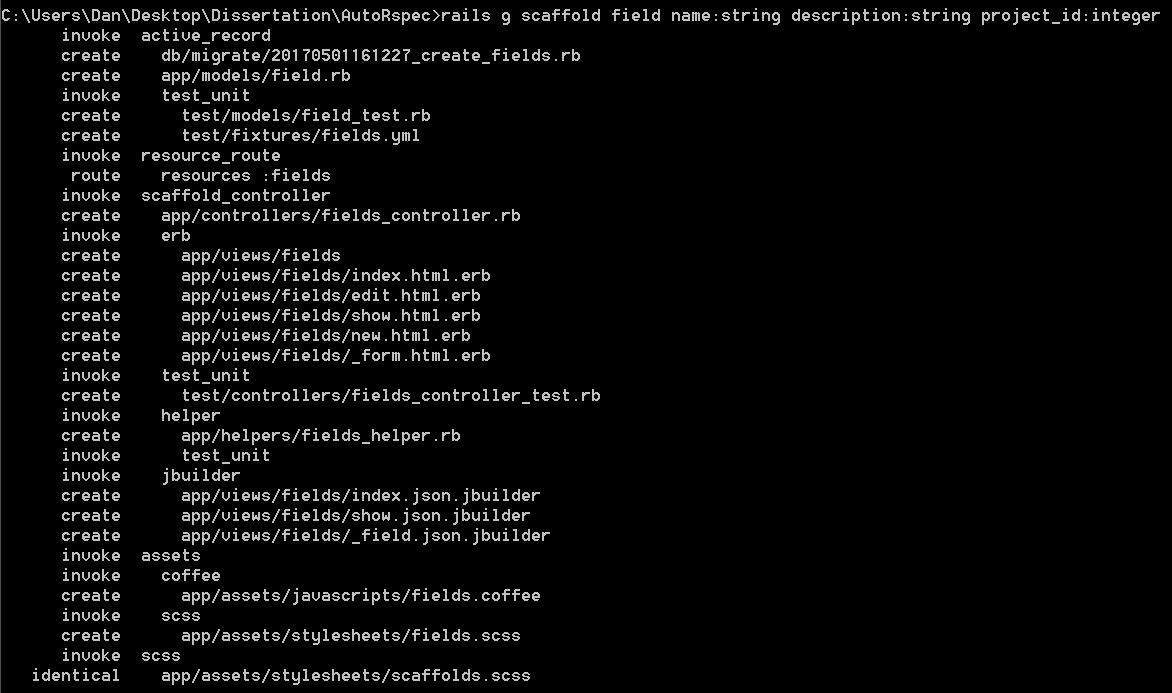
\includegraphics[width=\linewidth]{screenshots/scaffold_example}
\caption{Rails g scaffold command for field}
\label{fig:scaffold}
\end{figure}

\subsection{Database}

\par Rails natively supported active record assocations were used to establish the relations between the tables in the database\cite{railsara}\ref{fig:relations}. The dependent destroy option was used on relations where the deletion of the entity desired the deletion of entites that depended upon it outlined in the requirements, this will cause a cascade effect downwards through relations\ref{fig:relations}. Validations were applied intially according to the requirements then also dynamically throughout the process as they came relevant through implementation, e.g a fields name should follow the lower case underscore format that is convention in naming table fields in Ruby on Rails applications\ref{validations}. These validations were for the functionallity of the test suite generation and related functions.
\begin{figure}
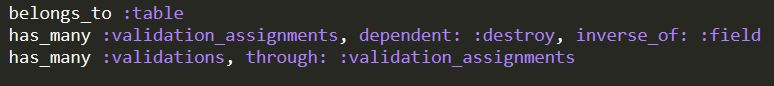
\includegraphics[width=\linewidth]{screenshots/relations}
\caption{Rails native relation methods used in field.rb model}
\label{fig:relations}
\end{figure}

\begin{figure}
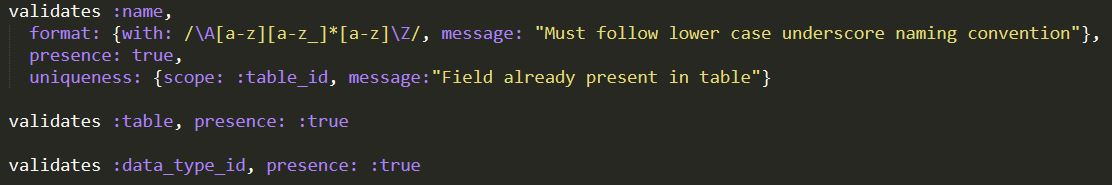
\includegraphics[width=\linewidth]{screenshots/validations}
\caption{Rails native validation method used in field.rb models}
\label{fig:validations}
\end{figure}



\subsection{View and Flow}
\par Bootstrap\cite{bootstrap} was used for the css of the web pages. Bootstrap gives a very clean and presentable wesbite by adding default css to HTML elements. Further classes that were used were table, table-hover, button classes and navbar classes. Bootstrap is extremely efficent for the view aspect of implementation. 
\par To get the flow outline in design the routes file had to be heavily configured. Rails reads the routes file from top to bottom, on the first path it hits that a match it will route to. Placing the custom routes above the nesting resources effectively overrides the defaults that rails will produce. The defaults needed to be overrode due to the nature of how when viewing an enity it displayed all of its dependent entities, aswell as being able to create a dependent entity. When the routes file had been configured rails it created the paths that could be used throughout the project\ref{fig:pathhelp}. The path helpers are desired as they take variables and produce a link thefore aid in the scaling and readablity of the project whilst also providing a very clear and methodical link.\cite{routing}



\begin{figure}
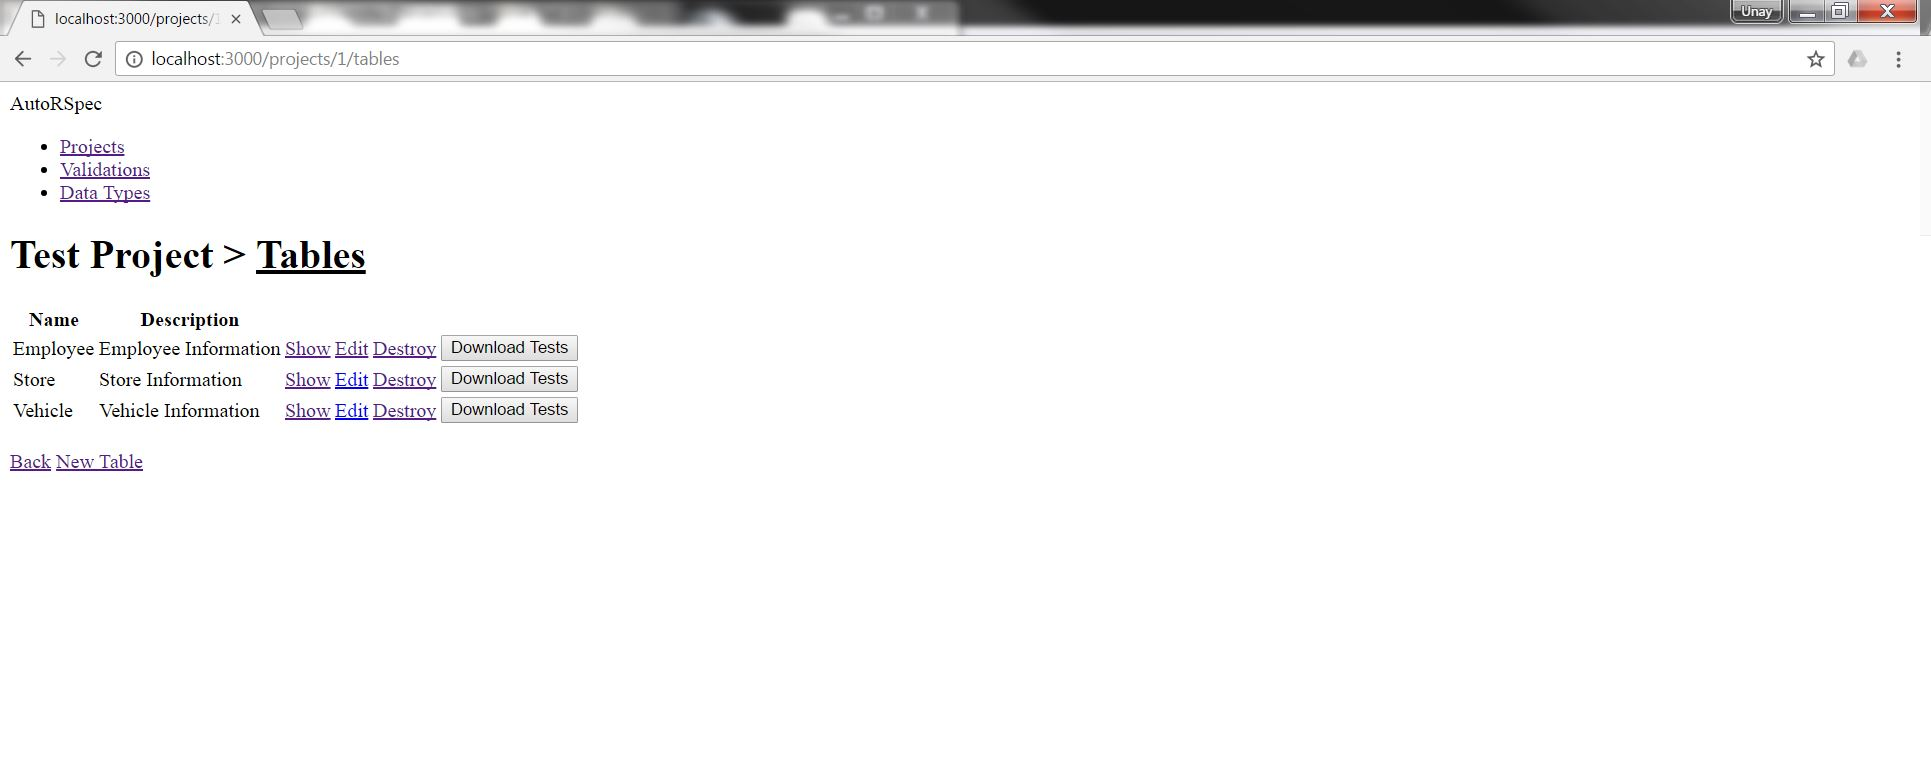
\includegraphics[width=\linewidth]{screenshots/nobootstrap}
\caption{Tables page without bootstrap}
\label{fig:nobootstrap}
\end{figure}

\begin{figure}
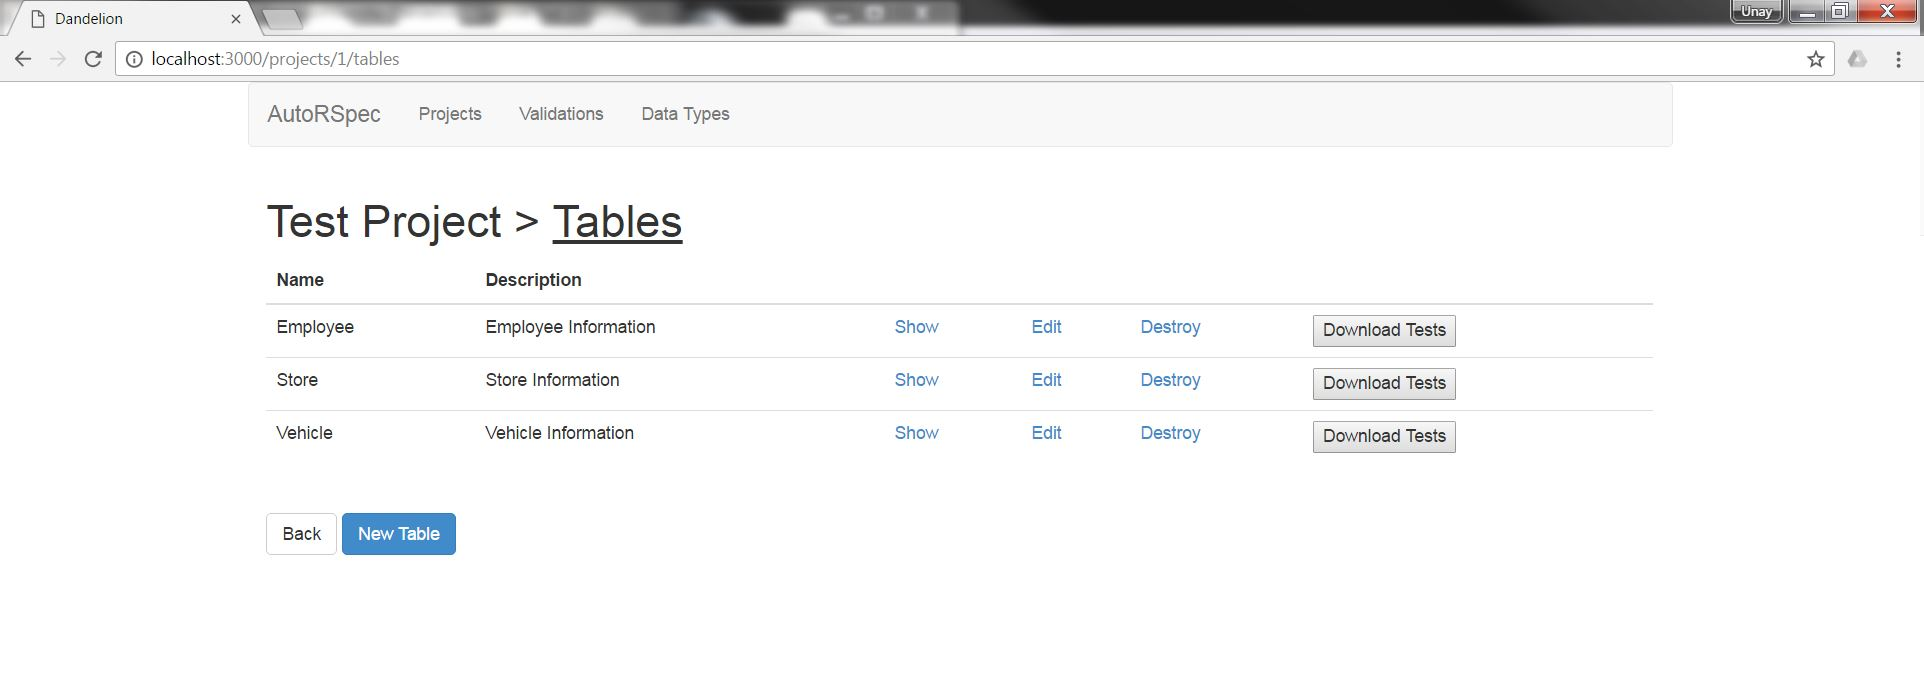
\includegraphics[width=\linewidth]{screenshots/bootstrap}
\caption{Tables page with bootstrap}
\label{fig:bootstrap}
\end{figure}

\begin{figure}
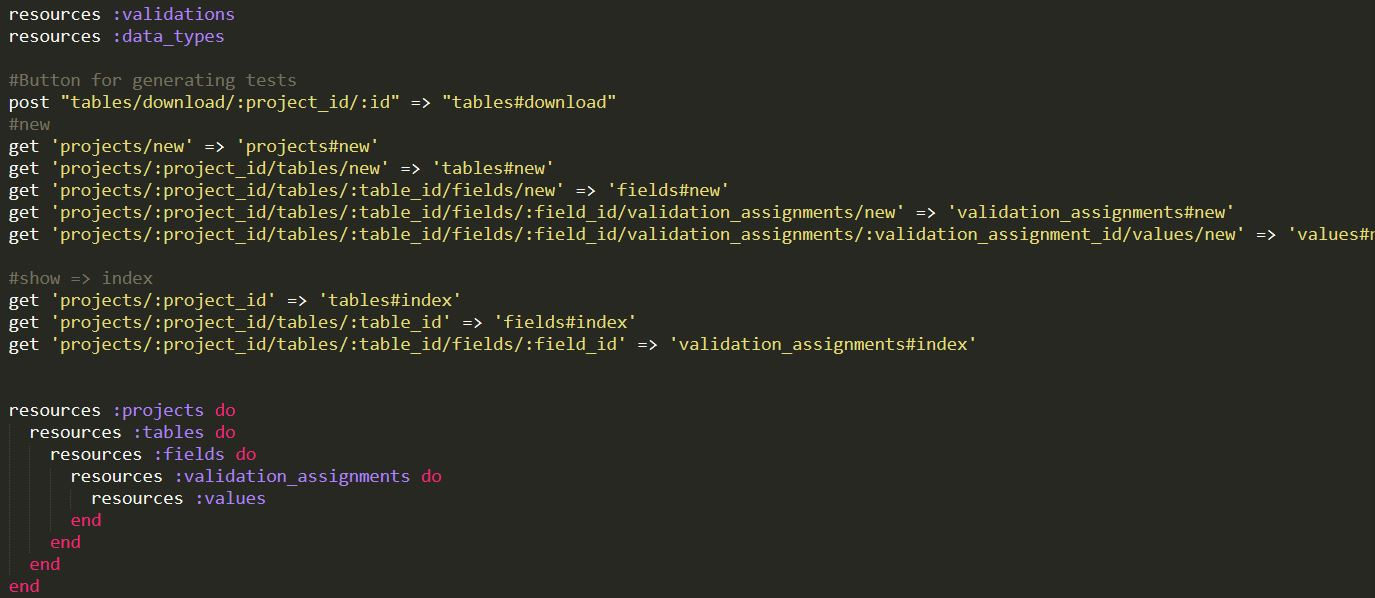
\includegraphics[width=\linewidth]{screenshots/routes}
\caption{Routes file for project}
\label{fig:routes}
\end{figure}

\begin{figure}
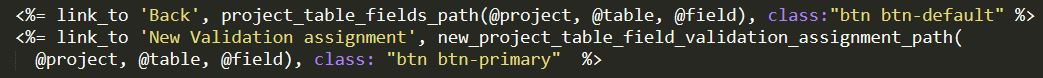
\includegraphics[width=\linewidth]{screenshots/root}
\caption{Example of path helper}
\label{fig:pathhelp}
\end{figure}

\subsection{Test Case Generation}


\subsubsection{Value Generation}

\par The design for generating a value was modified slightly due to finer details but its overall flow and princple was kept. One oversight from the design was the exclusion validation, when an exculsion validation is to be isolated it is logical to just return a random value from the list of values excluded as they will all fail the validation rather than try to randomly generate a value in the list.

\par \textbf{String Generation}

\par The generate\_string\_value function\ref{code:genstrval} is the top level function responsible for generating a string value for a test caseTo explain the function in depth the functions it uses will be explained first.

\begin{lstlisting}[frame=single,numbers=left,language = ruby,caption= {gen\_rand\_string\_array}, label={code:genranstr}]
def gen_rand_string_array(regex, amount)
  array = []
  # Generate amount specified as generated empty strings are deleted
  while array.length < amount
    string = regex.random_example(max_repeater_variance: 50)
    if string != ""
      array << string
    end
  end
  return array
end
\end{lstlisting}

\par \textbf{gen\_rand\_string\_array}\ref{code:genranstr}
\par gen\_rand\_string\_array takes two parameters regex and amount and returns an array of strings. regex is the regex from which the strings will be generated from and amount is the amount of strings to return in the array. The actual string value is generated using the 'regexp-examples'\cite{regexprangem} gem. The gem extends the regexp functionality by adding the function of generating a random string that is valid for that regular expression. The max\_repeater\_variable is set to 50, setting the amount of characters that can be included in the generated string output from each subsection of the regular expression pattern to be in the range of zero to fifty. The generated string can be an empty string so the generation is wrapped in a while loop to ensure the amount of strings returned is that of those requested in the parameters.

\begin{lstlisting}[frame=single,numbers=left,language = ruby,caption= {pass\_string\_rule}, label={code:passstrrule}]
def pass_string_rule( strings, rule, value )
  if rule == "regex"
    regex = value.to_regexp
    return strings.keep_if{ |n| n =~ regex } # =~ , ""[regex] , "".match(regex) #ATTN TIMINGS
  elsif rule == "exclusion"
    excluded = value.split(",").map(&:strip)
    return strings.delete_if{ |n| excluded.include?(n)}
  else # ASSUMED: Only length validations can progress to here
    # Comparorator stored as string in database e.g ">"
    return strings.keep_if{ |n| n.length.method(rule).(value.to_i)}
  end
end
\end{lstlisting}

\begin{lstlisting}[frame=single,numbers=left,language = ruby,caption= {fail\_string\_rule}, label={code:failstrrule}]
def fail_string_rule(strings, rule, value )
  if rule == "regex"
    regex = value.to_regexp
    return strings.delete_if{ |n| n =~ regex }
  else # ASSUMED: Only length validations can progress to here
    # Comparorator stored as string in database e.g ">"
    return strings.delete_if{ |n| n.length.method(rule).(value.to_i)}
  end
end
\end{lstlisting}


\par \textbf{pass\_string\_rule and fail\_string\_rule}
\par pass\_string\_rule takes three paramaters strings, rule and value and returns an array of strings. rule is the validation with value being the value of the validation, E.g rule = minimum length and value = 4, strings is the array of strings that have to pass the validation to be returned. The function starts by chechking if the rule is format validation, known internally as regex, if so it will remove any string form strings array parameter that does not meet the regular expression specified in the value parameter and return the array. Values are stored on the system database as strings so the 'to\_regexp' gem\cite{regexpstrgem} is used to convert the string into a regexp object.
\par Next it checks if the rule is exclusion, if so it will process the value parameter as seen on line 6 into an array of strings due to how its stored one string on the database. Then it will return the array of strings passed as the parameter with any string that is in the exclusion array removed. After these two checks the only validations that can remain for strings are length validations. Inclusion and blank are handled in another function and rule cannot be the exclusion or format validation. rule for length validations is a comparorator ( \textgreater=,\textgreater,==,\textless,\textless=) stored as a string in the database. This allows the functionallity of, return strings array parameter with strings kept if the the length of the string is 'rule' value. E.g keep if \textgreater 3.
\par fail\_string\_rule follows the same format as pass\_string\_rule with keep and delete string from string parameter array switched. fail\_rule\_string however does not have to check for exclusion as this is handled in generate\_string\_value.


\begin{lstlisting}[frame=single,numbers=left,language = ruby,caption= {prep\_string}, label={code:prepstr}]
def prep_string(string)
  # Add speech marks and escape \ " within to be written safely to test file
  return "\"" + string.gsub(/[\"\\]/){ |c| "\\"+c } + "\""
end
\end{lstlisting}

\par \textbf{prep\_string}
\par prep\_string takes a string and returns in with speech marks concated on each side and the '\textbackslash' and ' " ' characters escaped. It is used so when the string value is printed to file it is in the correct format and doesn't have any undesired effects that would occur if the characters were not escpaed.

\begin{lstlisting}[frame=single,numbers=left,language = ruby,caption= {generate\_string\_value}, label={code:genstrval}]
def generate_string_value(isolated, rest)
  # isolated can be passed as nil to generate a pass all
  # default regexp to generate strings
  regexp = [/\A[a-zA-Z]*[a-zA-Z]*\z/, /\A[\w]*[\w]*\z/, /\A[\w]*[[:punct:]]*[\w]*\z/, 
    /\A[\w]*[[:print:]]*[a-zA-Z]*\z/]
  # Add users regexp to the defaults if in rest
  if !rest.empty?
      if validations_contain?("format", rest)
        index = validations_index_of("format", rest)
        regexp << rest[index][1].to_regexp
      end
  end
  # Begin generation loop
  for full_iteration in 1..50
    strings = []
    # If testing exclusion then return one of its values 
    if (isolated != nil) && (isolated[0] == "exclusion")
      return prep_string(isolated[1].split(",").map(&:strip).sample) 
    else
      regexp.each do |r|
        strings += gen_rand_string_array(r, (1000/regexp.length))
      end
    end
    if isolated != nil
      strings = fail_string_rule(strings, isolated[0], isolated[1])
      if strings.empty?
        next
      end
    end
    rest.each do |rule|
      strings = pass_string_rule(strings, rule[0], rule[1])
      if strings.empty?
        break
      end
    end
    if strings.empty?
      next
    else
      return prep_string(strings.sample)
    end     
  end
  # No valid value generated
  return "\"!!!ERROR GENERATING VALUE\""
end
\end{lstlisting}

\par \textbf{generate\_string\_value}
\par The generate\_string\_value function\ref{code:genstrval} is the top level function responsible for generating a string value for a test case. It takes two parameters isolated and rest. isolated is the validation that has been isolated and is under test in the test case. rest are the other validations that are associated to the field under test. When both parameters are present it will return a string value that violates the isolated validation and obeys those in rest, rest can be an empty list. If isolated is nil it will return a string value that obeys all validation in rest. If a string value isnt generated it will return the string on line 43. 
\par At the begining of the function some regular expressions are defined in array, the regular expression decribe a diverse and varied range of patterns for strings. The function then checks to see if the validations to pass contain the format validation, if so it will concatenate the regular expression to those array defined previously. This is to include strings from the users format in the generation pool. After this check the iteration begins as described in the design chapter, the maximum iterations is fifty.
\par At the begining of the iteration an empty array is definfed call strings, this variable will contain the randomly generated strings to be processed. The first step of the iteration is to check if the isolated validation is 'exclusion', if so it will return a random tring from the array of excluded values stored in the database from the formal specifcation as they are the only strings that will fail the exclusion validation. This step could preceed the for loop but was included as it provides clarity having all validation handling within the iteraions, also it will only ever be ran once so no efficeny is lost. If exclusion is not the isolated validation then it will populate the strings array with randomly generated strings from the regular expressions 'regexp' defined above, generating 1000 strings in total with the same amount from each regular expression, giving wide range of diverse strings.
\par Once the strings have been generated the function checks if isolated is not nil, if so it will remove strings from the strings array that pass the isolated validation via fail\_string\_rule. Next it will iterate through each validation in rest and remove each string from strings array that fail the validation via pass\_string\_rule. Once all validations have been iterated through it will return a random value from strings array after preparing via prep\_string. Throughout the function after the strings array has been modified, strings potentailly removed, it will check if strings is empty and if so will 'next' to the next iteration. This is because strings is empty so no valid string remains so to increase efficency and save time it is logical to go to the next iteration.

\par \textbf{Number Generation}
\par Generating values for the float and integer datatypes follows the exact same methodolgy and structure as string. Therefore the slight differnce will be highlighted and infered as changes to generate\_string\_value. Numbers are randomly generated using rubys Random.rand with a range of negative one million to positive one million. The pass and fail rule functions dont have to account for the format validation but do have to account for divisible, which is accomplished by a map across the array of numbers. Also instead of comparing the length of a string with the comparorator the actual number is compared\ref{code:numsnip}. The last differnce is that the number returned does not need to be prepared like the string values.
\par The validators equal to and other than were removed as they are supported by creating a instance of inclusion or exclusion with one entry respectively. They were removed to reduce information overload for the user and reduce conflicting options

\begin{lstlisting}[frame=single,numbers=left,language = ruby,caption= {Differnce in pass/fail num rule to string pass/fail}, label={code:numsnip}]
if rule == "divisible"
  return numbers.keep_if{ |n| n % value == 0}
else # ASSUMED: Only >,>=,<,<= validations can progress to here
  # Comparorator stored as string in database e.g ">"
  return numbers.keep_if{ |n| n.method(rule).(value) }
end
\end{lstlisting}
\subsubsection{RSpec Test Case}

\par  In the design the behavioural description line of the RSpec test case, it "has this behaviour" do, was orginally in the test case template. However this was removed and is now handled by the test suite section, the change was to provide a more consistent test cases overall and make give the code greater clarity. Origanlly alot of variables were passed in through the hash and it made the template more complex and reduced its clarity, where as handling in test suite this problem was averted.

\par \textbf{test\_text}\ref{code:testtext}
\par test\_text is the template for all test cases apart from the specail case of blank test which is explained after this section. test\_text takes three parameters valid, hash and indent. valid is a boolean and is used to change the value of valid in the hash, this variable is a string that is repsonsible for the matcher "to" ot "to\_not" and is set according to the boolean, lines 3-7. hash is a hash that contains the necassary information to populate the template. The last parameter indent is the indentation the test case should start at. The function returns the string with the parts wrapped by \%\{ and \} replaced by the string value of the variable name in the hash. The hash is contructed in test suite and passed into test\_text as a parameter.
\begin{landscape}
\begin{lstlisting}[frame=single,numbers=left,language = ruby,caption= {test\_text}, label={code:testtext}]
def test_text(beValid,hash, indent)
  tab = "\t"
  if beValid
    hash[:valid] = "to"
  else
    hash[:valid] = "to_not"
  end
  template = tab*indent + "%{tableName} = build(:%{tableName}, %{fieldName}: %{generatedValue})\n" +
                   tab*indent + "if %{tableName}.respond_to?(:valid?)\n" +
                   tab*(indent+1) + "expect(%{tableName}).%{valid} be_valid, lambda {%{tableName}.errors.full_messages.join(\"\\n\")}\n" +
                   tab*indent + "end\n" 
  return template % hash
end
\end{lstlisting}
\end{landscape}

\par \textbf{blank\_test}\ref{code:blanktext}
\par The can be blank vaildator has its own template because the variations between the desired output and test\_text template were to great to make it clear and functional. The function follows the exact same methods, except it has a differn't template and it also contains the behaviour. 
\begin{landscape}
\begin{lstlisting}[frame=single,numbers=left,language = ruby,caption= {blank\_test}, label={code:blanktext}]
def blank_test(hash, bool, indent)
  tab = "\t" 
  template = tab*indent + "it \"%{decision} be blank\" do \n" +
             tab*(indent+1) + "%{tableName} = build(:%{tableName}, %{fieldName}: nil)\n" +
             tab*(indent+1) + "if %{tableName}.respond_to?(:valid?)\n" +
             tab*(indent+2) + "expect(%{tableName}).%{equator} be_valid, lambda {%{tableName}.errors.full_messages.join(\"\\n\")}\n" +
             tab*(indent+1) + "end\n" +
             tab*indent + "end\n\n"
  if bool
    hash[:decision] = "can"
    hash[:equator] = "to"
  else
    hash[:decision] = "can not"
    hash[:equator] = "to_not"
  end    
  return template % hash
end
\end{lstlisting}
\end{landscape}
\subsubsection{RSpec Test Suite}


\begin{lstlisting}[frame=single,numbers=left,language = ruby,caption= {generate\_tests\_for\_table}, label={code:bigboy}]
def generate_tests_for_table(id)

    table = Table.find(id)
    fileName = table.name.downcase + "_spec.rb"
    #file = File.open(fileName, "w")
    file = Tempfile.new(fileName,'tmp')
    # Introduction/Set-up file
    file.puts "require \"spec_helper\""
    file.puts ""
    file.puts "desrcibe \"" + table.name.titleize + "\" do"
    file.puts ""
    file << write_factory_test(table.name, 1)

    #Context loop for each field
    # Hash stores variables to populate test templates
    hash = { tableName: table.name.downcase}
    table.fields.each do |f|
      hash[:fieldName] = f.name
      if f.validation_assignments.empty?
        next 
      else
        file.puts "\tdescribe \"" + f.name + " field has validation\" do"
        file.puts ""
        validations = package_validations(f.validation_assignments)
        if validations_contain?("blank", validations)
          index = validations_index_of("blank", validations)
          if validations[index][1] == "true"
            file << blank_test(hash, true, 2)
          else
            file << blank_test(hash, false, 2)
          end
          # Remove blank from validations, fully handled
          validations.delete_at(index)
          hash.delete(:decision)
          hash.delete(:equator)
        end
        if validations_contain?("inclusion", validations)
          index = validations_index_of("inclusion", validations)
          if DataType.find(f.data_type_id).name == "String"
            stringArray = validations[index][1].split(",").map(&:strip)
            file << string_inclusion(hash, stringArray)
          else
            numberArray = database_string_to_number_array(validations[index][1])
            file << number_inclusion(hash, numberArray)
          end
          next # Inclusion supercedes remaining validations, skip to next
        end
        # test with all validations valid
        file.puts "\t\tit \"is valid with a generated value\" do\n"
        if DataType.find(f.data_type_id).name == "String"          
          value = generate_string_value(nil, validations)
          hash[:generatedValue] = value
          file << test_text(true, hash, 3)
        else
          value = 0
          if DataType.find(f.data_type_id).name == "Float"
            value = generate_value_integer(nil, validations, "Float")
          elsif DataType.find(f.data_type_id).name == "Integer"
            value = generate_value_integer(nil, validations, "Integer")
          end
          hash[:generatedValue] = value
          file << test_text(true, hash, 3)
        end
        # Write test isolating each validation to be invalid
        validations.each do |p|
          # Array we can manipulate
          rest = [].replace(validations)
          rest.delete_if{ |e| e == p} # remove isolated rule
          file.puts "\t\tit \"is invalid with value that is not " + p[0].to_s + " " + p[1].to_s + "\" do"
          if DataType.find(f.data_type_id).name == "String"
            value = generate_string_value(p, rest)
            hash[:generatedValue] = value
            file << test_text(false, hash, 3)
          else
            value = 0
            if DataType.find(f.data_type_id).name == "Float"
              value = generate_value_integer(nil, validations, "Float")
            elsif DataType.find(f.data_type_id).name == "Integer"
              value = generate_value_integer(nil, validations, "Integer")
            end
            hash[:generatedValue] = value
            file << test_text(false, hash, 3)
          end
          file.puts "\t\tend"
          file.puts ""
        end
      end
      file.puts "\tend"
      file.puts ""
    end
    file.puts "end"
    file.close
    return file.path, fileName
  end
\end{lstlisting}
\par \textbf{generate\_tests\_for\_table}\ref{code:bigboy}
\par generate\_tests\_for\_table is the function that takes on the responsiblities of test suite outlined in the design section. It takes the id of the table for which to generate the test suite for as a parameter an returns the file path and file name. When a user clicks the download link for a table is will invoke the download function, this invokes generate\_tests\_for\_table which using its return values the download function downloads the file to the user via the file path with the file name as file name.
\par The function begins by fetching the table from the database then creating the filename by taking the name of the table, downcasing it and concetaning '\_spec.rb' to it. Then a temporary file is created to write all of the information to, it creates a temporary file as it not needed locally for long as the user will download it once it has been generated. It then writes the necessary require and RSpec syntax to introduce the tables tests , lines 7-11. After this the factory test is wrote to the file, this is a simple test that makes sure the factory girl factory for the table the user has created is functioning correctly. The table name is then saved to a hash that will be used to store information for the test case tempaltes, this completes the preamble.
\par After the preammle the tables fields are iterated through. At the begining of each iteration the fields name is saved to the hash, then if the field has no validations it will 'next' to the next iteration. If there are validations it will write the RSpec syntax to introduce the field, lines 22-23. Next it will package the validations into a more manageable format as oppose to that stored on the database. Once packaged it will check if the validations contain the blank validation, if so it will write the blank test to the file using blank\_test and remove the validation from the packaged validations. 
\par The next check is for the inclusion validation and if it is present the data type appropiate function is called,explained after this section, to produce test cases which are added to the file then it 'next' to the next iteration. It skips the rest of the validations as inclusion supercedes all validations except blank, which is why blank precedes inlusion in order of checks in function. The next part in the function is to write a test case for where all validations are considered, this is to provide the information that the generation can create a valid value for all validations therfore making the isolated validations valid test cases, line 48-63. After it has been written to the file the next part is to iterate through each of the validaions. 
\par At the start of each iteration rest, an array that contains all other validations is created. Then the behavioural descriptor is wrote to the fiel, E.g it "is invalid with a value not less than 5" do. Depending on the data type of the field the appropiate value generation is called and saved to the has before calling test\_text which is written to the file. After each validation has been iterated through the function writes the correct syntax to the file to finish it then closes the file, then returns the path and filename.

\par \textbf{Inclusion}
\par Inclusion is handled seperatley as it supercedes other validations and has to be treated in a slightly differn't way due to the only values being accepted are those in the inclusion list. The possibilty of randomly generating a value that is in this list is too small to compute effeicently. Before calling the function generate\_test\_for\_table will convert the value string in the database to an array of the relevant data type. Number and string inclusion are dealt with in the same manner so only string inclusion will be explained in this document. 
\par string\_inclusion \ref{code:strinc} starts by storing in a variable a random value from the array of included values, this value will pass the validation. Then it will generate an array of random strings the same was as generate\_string\_value and remove any string from the array that is in inclusion, when a string is generated that is not included it is stored in a variable. Then it calls test\_text with the pssing variable and the valid boolean set to true to get a passing test case, after it calls it again the failing value and false, lines 18-21. After this it will concenate the test cases with there behavioural descriptors, lines 22-24, and return the string to generate\_test\_for\_table to be wrote to file.

\begin{lstlisting}[frame=single,numbers=left,language = ruby,caption= {generate\_tests\_for\_table}, label={code:strinc}]
def string_inclusion(hash, includedValues)
  correctValue = prep_string(includedValues.sample)
  incorrectValue = ""
  regexp = [/\A[a-zA-Z]*[a-zA-Z]*\z/, /\A[\w]*[\w]*\z/, /\A[\w]*[[:punct:]]*[\w]*\z/, /\A[\w]*[[:print:]]*[a-zA-Z]*\z/]
  strings = []
  for i in 1..50
    regexp.each do |r|
      strings += gen_rand_string_array(r, (1000/regexp.length))
    end
    strings.delete_if{ |n| includedValues.include?(n) }
    if strings.empty?
      next
    else
      incorrectValue = prep_string(strings.sample)
      break
    end
  end
  hash[:generatedValue] = correctValue
  correctTestText = test_text(true, hash, 3)
  hash[:generatedValue] = incorrectValue
  inCorrectTestText = test_text(false, hash, 3)
  correct_intro = "\t\tit \"is valid with a value from inclusion\" do\n"
  incorrect_intro = "\t\tit \"is invalid with a value not in inclusion\" do\n"
  return correct_intro + correctTestText + incorrect_intro + inCorrectTestText 
end
\end{lstlisting}

\subsection{Testing}

\par The first stage of testing was to set up the factories for the models using factory girl\cite{fgirl}. Factories allow for rapid and reliable testing using the once established factory to build a valid entity in test cases, seen on line 6 in Listing \ref{code:tabletests} . In fig \ref{code:fgirl} the factory for field is shown, the power of factory girl can be seen on line 5 where the table that field is dependent upon to be created can simple be defined by refering to the table factory. All model factories were constructed using the same method disaplyed in this example. Once the factories for each model had been defined RSpec test cases were written for requirements 1 to 12 of the functional specification requirements, see Table \ref{rq:1}, to test the functionality of the requirements, If a table can be edited and the edit is saved to the system. Table,  Listing \ref{code:tabletests}, and field, Listing \ref{code:fieldtests}, are included to show how an example of how all the rspec test cases were coded, the complete code in included in the online upload.
\par Once the tests had been written they could all be ran at once using the 'rspec spec/lib/*.rb', the asterix wild card runs all of the tests together. Twenty six test were ran all togther and they all passed, see Figure \ref{fig:mytestresult}. However this does not completely test the requirement as it is not performed by a user, to complete the testing for the requirement the system was used as a user would peform each action and the server log, see Listing \ref{code:deltab}, was read and database was queried, see Listing \ref{code:conex} to ensure the each requirements action were carried out. The server log shows the cascade of deletions carried out due to dependencies, the console query confirms the deletion of the table and fields, employee table is no longer in the database and there are no fields in the databse as all fields in the database belonged to the employee table. This method of simulating the user action, observing server logs and querying the database was taken as the manual method for testing.
\par  Requirements 13 to 16 of the functional specification requirements, see Table \ref{rq:1}, were tested manually. An example of how, A Project was navigated to using the website, the tables loaded in the browser, those loaded in the server logs and those queried in the console were all scrutinized to ensure that all tables for that project were loaded and only those tables. Requirement 5 in RSpec test suite \ref{rq:3} was also test using this manner.


\begin{figure}
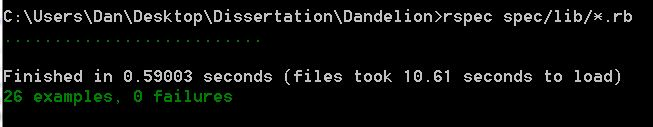
\includegraphics[width=\linewidth]{screenshots/mytestresult}
\caption{Cmd line ouput running all RSpec test on project}
\label{fig:mytestresult}
\end{figure}
\begin{lstlisting}[frame=single,numbers=left,language = ruby,caption= {Factory for field}, label={code:fgirl}]
FactoryGirl.define do
  factory :field do
    name { "field_" + random_word_lc }
    description "Dummy Information"
    table
    data_type_id 1
  end
end
def random_word_lc
  ('a'..'z').to_a.shuffle.join
end
\end{lstlisting}

\begin{lstlisting}[frame=single,numbers=left,language = ruby,caption= {RSpec tests for table}, label={code:tabletests}]
require "rails_helper"

describe Table do

  it "can be created" do
    table = create( :table)
    expect(Table.where(id: table.id).length).to eq(1)
  end
  
  it "can not be created without a project" do
    table = build( :table, project_id: 1)
    expect(table).to_not be_valid
  end

  it "can be edited" do
    table = create( :table, name:"Table")
    table.name = "Change"
    table.save
    expect(Table.where(id: table.id).first.name).to eq("Change")
  end

  it "can be deleted" do
    table = create( :table)
    table.destroy
    expect(Table.where(id: table.id).length).to eq(0)
  end

  it "deletes associated tables when deleted" do
    table = create( :table)
    field = create(:field, table_id: table.id)
    table.destroy
    expect(Field.where(id: field.id).length).to eq(0)
  end

end
\end{lstlisting}
\begin{lstlisting}[frame=single,numbers=left,language = ruby,caption= {RSpec tests for field}, label={code:fieldtests}]
require "rails_helper"

describe Field do

  it "can be created" do
    field = create( :field)
    expect(Field.where(id: field.id).length).to eq(1)
  end
  
  it "can not be created without a project" do
    field = build( :field, table_id: 1)
    expect(field).to_not be_valid
  end

  it "can be edited" do
    field = create( :field, name:"field")
    field.name = "change"
    field.save
    expect(Field.where(id: field.id).first.name).to eq("change")
  end

  it "can be deleted" do
    field = create( :field)
    field.destroy
    expect(Field.where(id: field.id).length).to eq(0)
  end

  it "deletes associated fields when deleted" do
    field = create( :field)
    validation_assignment = create(:validation_assignment, field_id: field.id)
    field.destroy
    expect(ValidationAssignment.where(id: validation_assignment.id).length).to eq(0)
  end

  it "can have a given validation" do
    field = create( :field)
    validation = create(:validation)
    validation_assignment = create(:validation_assignment, field_id: field.id,
      validation_id: validation.id)
    expect(ValidationAssignment.where(id: validation_assignment.id).first.field_id).to eq(field.id)
  end

end
\end{lstlisting}

\begin{table}
\centering
\caption{Formal Specification Requirements Testing}
\label{met:1}
\begin{tabularx}{\textwidth}{|l|X|l|l|}
\hline
\textbf{ID} & \textbf{Requirement}                                                   & \textbf{Written} & \textbf{Manual} \\ \hline
\textbf{1}  & A user can create a Project                                            & \textbf{Y} & \textbf{Y}       \\ \hline
\textbf{2}  & A user can edit a Project                                              & \textbf{Y}  & \textbf{Y}      \\ \hline
\textbf{3}  & A user can delete a Project, associated Tables are also deleted        & \textbf{Y}  & \textbf{Y}      \\ \hline
\textbf{4}  & A user can create a Table, only for a given  Project                   & \textbf{Y}  & \textbf{Y}      \\ \hline
\textbf{5}  & A user can edit a Table                                                & \textbf{Y}     & \textbf{Y}   \\ \hline
\textbf{6}  & A user can delete a Table, associated Fields are also deleted          & \textbf{Y} & \textbf{Y}       \\ \hline
\textbf{7}  & A user can create a Field, only for a given Table                      & \textbf{Y}   & \textbf{Y}     \\ \hline
\textbf{8}  & A user can edit a Field                                                & \textbf{Y}    & \textbf{Y}    \\ \hline
\textbf{9}  & A user can delete a Field, associated validations are also deleted     & \textbf{Y}      & \textbf{Y}  \\ \hline
\textbf{10} & A user can assign a validation, only for a given Field       & \textbf{Y}    & \textbf{Y}    \\ \hline
\textbf{11} & A user can only create a value for a assigned validation                  & \textbf{Y}      & \textbf{Y}  \\ \hline
\textbf{12} & A user can edit a  value                      & \textbf{Y}     & \textbf{Y}   \\ \hline
\textbf{13} & A user can view all Projects                 & \textbf{N}   & \textbf{Y}     \\ \hline
\textbf{14} & A user can view all Tables associated to a given Project               & \textbf{N}   & \textbf{Y}     \\ \hline
\textbf{15} & A user can view all Fields associated to a given Table                 & \textbf{N}   & \textbf{Y}     \\ \hline
\textbf{16} & A user can view all validations and values associated to a given field & \textbf{N}    & \textbf{Y}    \\ \hline
\end{tabularx}
\end{table}

see Listing \ref{code:nice} see Figure \ref{rspecfail}

\par Test case requirements, table \ref{met:2}, 1-3,5,7-12 were proved met by the Project suite, Listing \ref{code:nice} being able to run and also demonstrating being able to describe a specfifc failure occuring,  see Figure \ref{fig:rspecfailcode}. All requirements 2-12 can be observed by inspecting the Project suite, while subjective to the person inspecting there is enough evidence to justify each requirement. For example 4 and 6 require human readable text, the test cases are understandable and the behaviour under test can be inferred by reading the source code of the test cases aswell as when they are ran. 7-12 can be observed by reading the validations under test and calculating if the generated value is correct.

\begin{table}
\centering
\caption{RSpec Test Case Requirements Testing}
\label{met:2}
\begin{tabularx}{\textwidth}{|l|X|l|l|}
\hline
\textbf{ID} & \textbf{Requirement}                                                                                                                       & \textbf{Written} & \textbf{Manual}  \\ \hline
\textbf{1}  & RSpec test case should be runnable                                                                                                         & \textbf{N}   & \textbf{Y}     \\ \hline
\textbf{2}  & RSpec test case should only test one behaviour                                                                                             & \textbf{N}   & \textbf{Y}       \\ \hline
\textbf{3}  & RSpec test case must should test behaviour intended                                                                                    & \textbf{N}   & \textbf{Y}        \\ \hline
\textbf{4}  & RSpec descriptor must be human readable                                                                                                    & \textbf{N}   & \textbf{Y}       \\ \hline
\textbf{5}  & When test case fails, its output must specify exact behaviour at fault                                                                     & \textbf{N}   & \textbf{Y}    \\ \hline
\textbf{6}  & RSpec test case should have human readable syntax                                                                                & \textbf{N}   & \textbf{Y}     \\ \hline
\textbf{7}  & Be able to generate an Integer that satisfies all validations and their values assigned to a field                                         & \textbf{N}   & \textbf{Y}       \\ \hline
\textbf{8}  & Be able to generate an Integer that does not satisfy a validation but satisfies all other validations and their values assigned to a field  & \textbf{N}   & \textbf{Y}       \\ \hline
\textbf{9}  & Be able to generate a Float that satisfies all validations and their values assigned to a field                                             & \textbf{N}   & \textbf{Y}       \\ \hline
\textbf{10} & Be able to generate a Float that does not satisfy a validation but satisfies all other validations and their values assigned to a field    & \textbf{N}   & \textbf{Y}  \\ \hline
\textbf{11} & Be able to generate a String that satisfies all validations and their values assigned to a field                                            & \textbf{N}   & \textbf{Y}       \\ \hline
\textbf{12} & Be able to generate a String that does not satisfy a validation but satisfies all other validations and their values assigned to a field    & \textbf{N}   & \textbf{Y}      \\ \hline
\end{tabularx}
\end{table}

\par Analysing a test suite, Listing \ref{code:nice}, produced for Products, defined in chapter 6, it can be concluded that the test cases are grouped via field and in a logical order, passing requirements 3,4 for Test suite, table \ref{met:3}. Querying the database and cross refrencing the fields and validations belonging to products between those tested in the suite requirement 2 can be confirmed to met aswell. The final requirement, 1, was validated as met by running the test suite, figure \ref{fig:runsuite}.

\begin{figure}
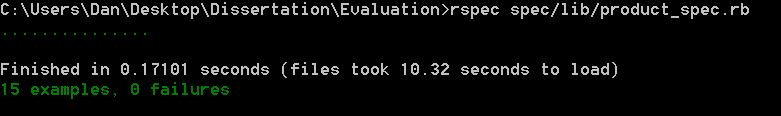
\includegraphics[width=\linewidth]{screenshots/runsuite}
\caption{Result of running Product test suite}
\label{fig:runsuite}
\end{figure}

\begin{table}
\centering
\caption{RSpec Test Suite Requirements Testing}
\label{met:3}
\begin{tabularx}{\textwidth}{|l|X|l|l|}
\hline
\textbf{ID} & \textbf{Requirement}                                          & \textbf{Written} & \textbf{Manual} \\ \hline
\textbf{1}  & RSpec test suite should be runnable                          & \textbf{N}   & \textbf{Y}       \\ \hline
\textbf{2}  & RSpec test suite should be contain all test cases for a table  & \textbf{N}   & \textbf{Y}      \\ \hline
\textbf{3}  & RSpec test cases should be grouped via field                 & \textbf{N}   & \textbf{Y}      \\ \hline
\textbf{4}  & RSpec test cases should be in a logical order                 & \textbf{N}   & \textbf{Y}      \\ \hline
\textbf{5}  & RSpec test suite must be available for download               & \textbf{N}   & \textbf{Y}     \\ \hline
\end{tabularx}
\end{table}

\par All requirements were concluded to be met, however the majority of these were done manually can can be subjective. The output of the system is fully functional and serves the purpose it intended to.


\section{Chapter 6: Results and Discussion}

\subsection{Evaluation Subject Requirements}
\par For evaluation the following three criteria were desired, all three were not necessary but these were the main factors in choosing subjects. The criteria was chosen to similute useage of the system as close as possible and to provide the best results for analysis.
\begin{enumerate}
\item \textbf{A Specfication}
\par A description of the intended program behaviour that was seperate from the code such as a design specification from which to construct the functional specification using the system. This mimics how a user will use the system.
\item \textbf{Database}
\par To use a mixture of validations supported and not supported on the data types supported and also have a range of table sizes. Provide a range of results for analysis.
\item \textbf{Test cases}
\par Have an already established suite of test cases, preferably RSpec to compare with. To compare results and analyse efficency and effectiveness.
\end{enumerate}

\cite{near2012rubicon}
\cite{near2014derailer}
\par Redmine, Fat Free CRM, Dispora, Amahi and Selfstarter from Derailer\cite{near2014derailer} and Inoshi, RubyTime, RubyURL and Tracks from Rubicon\cite{near2012rubicon} evaluation subjects were considered but none of them met the desried criteria to a high enough level. Therefore four tables will be constructed to be evaluated. The three tables will range in size, data types used and validations. The specification for the tables to be created are as follows:

\par \textbf{Product}
\begin{enumerate}
\item code : Integer
\par  Cannot be blank, greater than 0, less than 10000 
\item name : String
\par Can be blank, format /{\textbackslash}A[a-zA-Z]+{\textbackslash}z/
\item stock : Integer 
\par Cannot be blank, greater than or equal to 0, divisible by 5
\item price : Float 
\par Cannot be blank, greater than 0, less than 10000 
\end{enumerate}

\par \textbf{Employee}
\begin{enumerate}
\item Title : String 
\par Can be blank, Inclusion [ Miss, Mrs, Mr, Dr, Prof ]
\item first\_name : String
\par  minimum length 5 
\item last\_name : String
\par cannot be blank, maximum length 20
\item position : String 
\par Cannot be blank, Exclusion [ Boss, CEO ]
\item age : Integer 
\par greater than or equal to 0, less than or equal to 100
\item hourly\_pay : Float 
\par greater than or equal to 6.12, exclusion[ 23.45]
\end{enumerate}

\par \textbf{Account}
\begin{enumerate}
\item account\_type : Integer
\par  Can be blank, divisible by 63
\item name : String
\par Can be blank, format /{\textbackslash}A[a-zA-Z]+[\_][a-zA-Z]+{\textbackslash}z/
\item rating : float 
\par Cannot be blank, less than 10000, divisible by 0.1

\end{enumerate}

\par Once the specifcations were entered and generated, producing a total of 44 test cases for all three tables . The tests were ran there was one failure. This was the system failing to produce a float that isloated the less than 10000 field on table Account, see Figure \ref{fig:rspecfail}. However on looking at the test it is clear the test is at fault and not the users sytem under test with the error message in place of the value, see Figure \ref{fig:rspecfailcode}.

\par For the first part of the evaluation mutation testing will be used, validations will be removed, altered and added and the test suites will be ran, this will demonstrate wether the test suites can pick up the missing validation. A Y in the detected column indicates the tests detected the change, whereas an N indicates they did not.

\begin{table}
\centering
\caption{Mutation Testing}
\label{test:1}
\begin{tabularx}{\textwidth}{|l|X|l|l|}
\hline
\textbf{ID} & \textbf{Change}                                          & \textbf{Detected} \\ \hline
\textbf{1}  & Divisible by 63 removed from Account, account\_type                       & \textbf{Y}\\ \hline
\textbf{2}  & Divisible by 63 changed to 79 from Account, account\_type                       & \textbf{N}\\ \hline
\textbf{3}  & Can be blank changed to can not, from Account, account\_type                       & \textbf{Y}\\ \hline
\textbf{4}  & Tests 1 and 3 at the same time                       & \textbf{Y}\\ \hline
\textbf{5}  & Greater than or equal to 0 removed from Product, stock & \textbf{Y}     \\ \hline
\textbf{6}  & Exclusion removed from Employee, position                 & \textbf{Y}   \\ \hline
\textbf{7}  & Exclusion and maximum length from Employee, position, last\_name               & \textbf{Y}     \\ \hline
\textbf{8}  & Format /{\textbackslash}A[a-zA-Z]+{\textbackslash}z/added to Employee, first\_name              & \textbf{Y}       \\ \hline
\textbf{9}  & Minimum Length 10 added to  Account, name             & \textbf{N}       \\ \hline
\textbf{10}  & Uniqueness true  added to  Product, code             & \textbf{N}       \\ \hline
\end{tabularx}
\end{table}

\begin{figure}
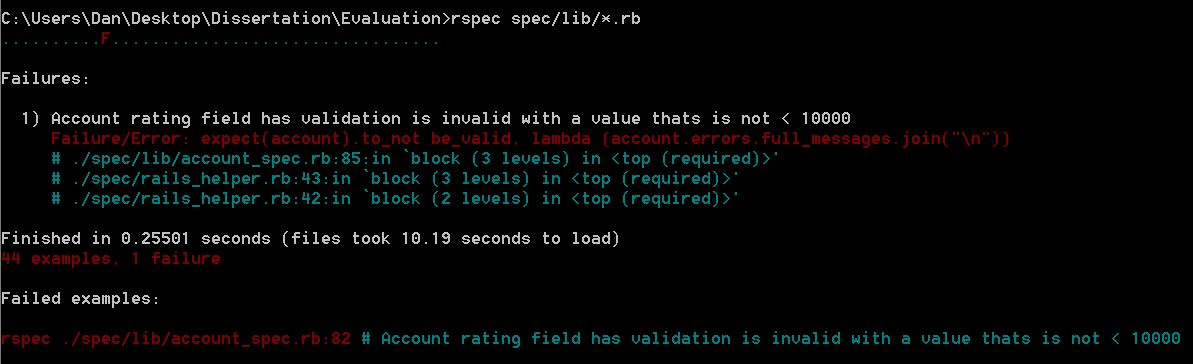
\includegraphics[width=\linewidth]{screenshots/rspecfail}
\caption{An example of a failing Rspec test case produced by the system}
\label{fig:rspecfail}
\end{figure}

\begin{figure}
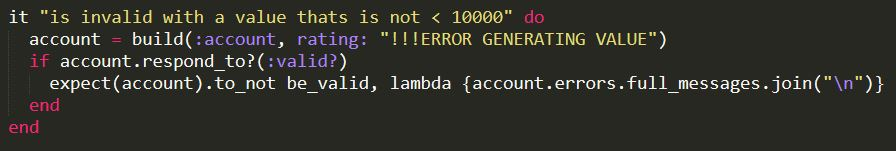
\includegraphics[width=\linewidth]{screenshots/rspecfailcode}
\caption{An example of a test case where a value could not be generated}
\label{fig:rspecfailcode}
\end{figure}

\par For the second part of mutation testing the potentail effectiveness of using the system was evaluated.
\par It took three minutes thirty seconds to construct the formal specifcation for Project, three minute fifty five seconds for Employee and two minutes and sixteen seconds for Account. Giving a total of nine minutes and thrity six seconds to construct the functional specifications on the system. The total test cases produced in all three suites was forty four, with one having not been able to generate a value, so forty three test cases. These forty three test cases  were ran and all had the desried behaviour. This gives an average of thirteen seconds to produce a valid working test case, which is a credible speed and is certainly faster than the time it takes to produce a manually written test case.
\par The test suite and individual test cases, see Figure \ref{code:nice}, showed good readability and could be understood to a standard high enough to locate the behaviour at fault. The layout and overall structure is logical and is as expected. Thes factors show that the test suite produced could serve as an initail test file and a foundation for which more complex test are added to. The suite would be useful as the initail tests in a test driven development style of development.


\section{Chapter 7: Conclusions}

\subsection{System}

\subsubsection{Improvements to current system}

\par Some improvements that could be made to the current system are:
\begin{enumerate}
\item Level of user freindliness
\par Currently there are no restrictions on what combinations of validations can be chosen, this allows the user to set fields with validations that have no possible valid value. This was an oversight as it was expected a user had a well designed and defined specfication. The current error handling for not generating a value is to return a string that has high visibility, this was to ensure the test suite was still generated, an improvement could be prompting the user with an error message. Navigating over two layers, e.g from value to table consists of clicking back multiple time or project then table, having the hierachy line that describes the current position as linkable, E.g can click on the table name to go to the table would improve navigation.
\item Border cases for numerical tests
\par Border case testing, testing 9, 10, 11 for a maximum value of 10 on a validation is a standard usually followed in automated testing but not in RSpec test cases. This could be introduced as a feature that could be toggled, some users may not want it as it would produce a lot of test cases they may not want.
\item Database fetching efficency
\par There a few difffern't ways of fetching data from the database in ruby. One method that isnt implemented fetches all relevant entries and stores them in cache, which can be queried further on, reducing the amount of calls to the database. The differn't methods could be consulted for each fecth to increase optimisation.
\end{enumerate}

\subsubsection{System Expandability}
\par Import, Export, Use it

\begin{enumerate}
\item more validations
\item relations
\item more data types
\item generating customisabel/ all tables etc etc
\item could use knowledge to produce factory girl skeletons
\end{enumerate}
\subsection{Conclusion}

\par This project started out with the motivation of bringing the benefits of automated testing to Ruby on Rails. Through research it was discovered there is automated testing but it does not fit with the Test Driven  and iterational style of testing that Ruby on Rails encourages and is practiced in development of its applications. The aim was refined to creating a system that automatically generates RSpec test cases for model validation in Ruby on Rails Applications. This refined aim fit the natural development cycle of Ruby on Rails applications by automating the writing of test cases that will be written manually by a developer. The test suite generated is basic, that is it only tests for the validations attached to fields. It does however serve as a good foundation from which to add test cases to and as the start of testing in the development cycle.

\appendix
\begin{lstlisting}[frame=single,numbers=left,,caption= {Server log for deleting Employee table}, label={code:deltab}]
#destroy as HTML
oken"=>"tJA1Mc52lZYdmAqYnAQqOtpMpZvKp8LS/0yVeb4nAmvlj2T26Mo8sHqAFNmc78TPNEwDB0ET4xY5fDeddcrKsg==", "project_id"=>"1",

  "projects".* FROM "projects" WHERE "projects"."id" = ? LIMIT 1  [["id", 1]]
"tables".* FROM "tables" WHERE "tables"."project_id" = ? AND "tables"."id" = ? LIMIT 1  [["project_id", 1], ["id", 1]]

fields".* FROM "fields" WHERE "fields"."table_id" = ?  [["table_id", 1]]
.0ms)  SELECT "validation_assignments".* FROM "validation_assignments" WHERE "validation_assignments"."field_id" = ?

"values".* FROM "values" WHERE "values"."validation_assignment_id" = ? LIMIT 1  [["validation_assignment_id", 3]]
lues" WHERE "values"."id" = ?  [["id", 3]]
lidation_assignments" WHERE "validation_assignments"."id" = ?  [["id", 3]]
"values".* FROM "values" WHERE "values"."validation_assignment_id" = ? LIMIT 1  [["validation_assignment_id", 5]]
lues" WHERE "values"."id" = ?  [["id", 5]]
lidation_assignments" WHERE "validation_assignments"."id" = ?  [["id", 5]]
"values".* FROM "values" WHERE "values"."validation_assignment_id" = ? LIMIT 1  [["validation_assignment_id", 6]]
lues" WHERE "values"."id" = ?  [["id", 6]]
lidation_assignments" WHERE "validation_assignments"."id" = ?  [["id", 6]]
"values".* FROM "values" WHERE "values"."validation_assignment_id" = ? LIMIT 1  [["validation_assignment_id", 7]]
lues" WHERE "values"."id" = ?  [["id", 7]]
lidation_assignments" WHERE "validation_assignments"."id" = ?  [["id", 7]]
elds" WHERE "fields"."id" = ?  [["id", 1]]
.0ms)  SELECT "validation_assignments".* FROM "validation_assignments" WHERE "validation_assignments"."field_id" = ?

"values".* FROM "values" WHERE "values"."validation_assignment_id" = ? LIMIT 1  [["validation_assignment_id", 8]]
lues" WHERE "values"."id" = ?  [["id", 8]]
lidation_assignments" WHERE "validation_assignments"."id" = ?  [["id", 8]]
"values".* FROM "values" WHERE "values"."validation_assignment_id" = ? LIMIT 1  [["validation_assignment_id", 9]]
lues" WHERE "values"."id" = ?  [["id", 9]]
lidation_assignments" WHERE "validation_assignments"."id" = ?  [["id", 9]]
elds" WHERE "fields"."id" = ?  [["id", 2]]
.0ms)  SELECT "validation_assignments".* FROM "validation_assignments" WHERE "validation_assignments"."field_id" = ?

"values".* FROM "values" WHERE "values"."validation_assignment_id" = ? LIMIT 1  [["validation_assignment_id", 1]]
lues" WHERE "values"."id" = ?  [["id", 1]]
lidation_assignments" WHERE "validation_assignments"."id" = ?  [["id", 1]]
"values".* FROM "values" WHERE "values"."validation_assignment_id" = ? LIMIT 1  [["validation_assignment_id", 2]]
lues" WHERE "values"."id" = ?  [["id", 2]]
lidation_assignments" WHERE "validation_assignments"."id" = ?  [["id", 2]]
"values".* FROM "values" WHERE "values"."validation_assignment_id" = ? LIMIT 1  [["validation_assignment_id", 10]]
lues" WHERE "values"."id" = ?  [["id", 10]]
lidation_assignments" WHERE "validation_assignments"."id" = ?  [["id", 10]]
"values".* FROM "values" WHERE "values"."validation_assignment_id" = ? LIMIT 1  [["validation_assignment_id", 11]]
lues" WHERE "values"."id" = ?  [["id", 11]]
lidation_assignments" WHERE "validation_assignments"."id" = ?  [["id", 11]]
"values".* FROM "values" WHERE "values"."validation_assignment_id" = ? LIMIT 1  [["validation_assignment_id", 12]]
lues" WHERE "values"."id" = ?  [["id", 12]]
lidation_assignments" WHERE "validation_assignments"."id" = ?  [["id", 12]]
elds" WHERE "fields"."id" = ?  [["id", 3]]
.0ms)  SELECT "validation_assignments".* FROM "validation_assignments" WHERE "validation_assignments"."field_id" = ?

"values".* FROM "values" WHERE "values"."validation_assignment_id" = ? LIMIT 1  [["validation_assignment_id", 13]]
lues" WHERE "values"."id" = ?  [["id", 13]]
lidation_assignments" WHERE "validation_assignments"."id" = ?  [["id", 13]]
"values".* FROM "values" WHERE "values"."validation_assignment_id" = ? LIMIT 1  [["validation_assignment_id", 14]]
lues" WHERE "values"."id" = ?  [["id", 14]]
lidation_assignments" WHERE "validation_assignments"."id" = ?  [["id", 14]]
"values".* FROM "values" WHERE "values"."validation_assignment_id" = ? LIMIT 1  [["validation_assignment_id", 15]]
lues" WHERE "values"."id" = ?  [["id", 15]]
lidation_assignments" WHERE "validation_assignments"."id" = ?  [["id", 15]]
elds" WHERE "fields"."id" = ?  [["id", 4]]
bles" WHERE "tables"."id" = ?  [["id", 1]]

:3000/projects/1
ctiveRecord: 13.0ms)
\end{lstlisting}
\begin{lstlisting}[frame=single,numbers=left,language = ruby,caption= {Rails console query for table and field existance}, label={code:conex}]
::1 at 2017-05-03 01:17:12 +0100
#index as HTML
1"}
  "projects".* FROM "projects" WHERE "projects"."id" = ? LIMIT 1  [["id", 1]]
tables".* FROM "tables" WHERE "tables"."project_id" = ?  [["project_id", 1]]
rb within layouts/application (3.0ms)
s: 63.0ms | ActiveRecord: 0.0ms)

irb(main):011:0> Table.all  
 Table Load (1.0ms)  SELECT "tables".* FROM "tables"     => #<ActiveRecord::Relation [#<Table id: 2, name: "Store", description: "Store Information", project_id: 1, created_at: "2017-04-24 22:17:38", updated_at: "2017-04-24 22:17:38">, #<Table id: 3, name: "Vehicle", description: "Vehicle Information", project_id: 1, created_at: "2017-04-24 22:17:38", updated_at: "2017-04-24 22:17:38">]> 
irb(main):012:0> Field.all
 Field Load (0.0ms)  SELECT "fields".* FROM "fields" => #<ActiveRecord::Relation []> 
\end{lstlisting}

\begin{lstlisting}[frame=single,numbers=left,language = ruby,caption= {Test suite output for Product defined in chapter 6}, label={code:nice}]
require "rails_helper"

describe Product do

	it "has a valid factory" do
		expect(build(:product)).to be_valid
	end

	describe "code field has validation" do

		it "can not be blank" do 
			product = build(:product, code: nil)
			if product.respond_to?(:valid?)
				expect(product).to_not be_valid, lambda {product.errors.full_messages.join("\n")}
			end
		end

		it "is valid with a generated value" do
			product = build(:product, code: 9314)
			if product.respond_to?(:valid?)
				expect(product).to be_valid, lambda {product.errors.full_messages.join("\n")}
			end
		end

		it "is invalid with a value thats is not > 0" do
			product = build(:product, code: -487078)
			if product.respond_to?(:valid?)
				expect(product).to_not be_valid, lambda {product.errors.full_messages.join("\n")}
			end
		end

		it "is invalid with a value thats is not < 10000" do
			product = build(:product, code: 449752)
			if product.respond_to?(:valid?)
				expect(product).to_not be_valid, lambda {product.errors.full_messages.join("\n")}
			end
		end

	end

	describe "name field has validation" do

		it "can be blank" do 
			product = build(:product, name: nil)
			if product.respond_to?(:valid?)
				expect(product).to be_valid, lambda {product.errors.full_messages.join("\n")}
			end
		end

		it "is valid with a generated value" do
			product = build(:product, name: "XoJbfmoPkAHFv")
			if product.respond_to?(:valid?)
				expect(product).to be_valid, lambda {product.errors.full_messages.join("\n")}
			end
		end

		it "is invalid with a value thats is not regex /\A[a-zA-Z]+\z/" do
			product = build(:product, name: "CaQEWaIldTMdNiNN!'}??-@)&\"(-'*:]!'(FnahDn8DrLNY6_5u04e0jrEPQJmWX")
			if product.respond_to?(:valid?)
				expect(product).to_not be_valid, lambda {product.errors.full_messages.join("\n")}
			end
		end

	end

	describe "stock field has validation" do

		it "can not be blank" do 
			product = build(:product, stock: nil)
			if product.respond_to?(:valid?)
				expect(product).to_not be_valid, lambda {product.errors.full_messages.join("\n")}
			end
		end

		it "is valid with a generated value" do
			product = build(:product, stock: 902865)
			if product.respond_to?(:valid?)
				expect(product).to be_valid, lambda {product.errors.full_messages.join("\n")}
			end
		end

		it "is invalid with a value thats is not >= 0" do
			product = build(:product, stock: -140355)
			if product.respond_to?(:valid?)
				expect(product).to_not be_valid, lambda {product.errors.full_messages.join("\n")}
			end
		end

		it "is invalid with a value thats is not divisible 5" do
			product = build(:product, stock: 587473)
			if product.respond_to?(:valid?)
				expect(product).to_not be_valid, lambda {product.errors.full_messages.join("\n")}
			end
		end

	end

	describe "price field has validation" do

		it "is valid with a generated value" do
			product = build(:product, price: 5563.56)
			if product.respond_to?(:valid?)
				expect(product).to be_valid, lambda {product.errors.full_messages.join("\n")}
			end
		end

		it "is invalid with a value thats is not > 0" do
			product = build(:product, price: -67150.92)
			if product.respond_to?(:valid?)
				expect(product).to_not be_valid, lambda {product.errors.full_messages.join("\n")}
			end
		end

		it "is invalid with a value thats is not < 10000" do
			product = build(:product, price: 59127.4)
			if product.respond_to?(:valid?)
				expect(product).to_not be_valid, lambda {product.errors.full_messages.join("\n")}
			end
		end

	end

end
\end{lstlisting}

\bibliography{bibliography}
\bibliographystyle{ieeetr}
\end{document}
